\chapter{Klassische Mechanik}

\section{Abriss der Newtonsche Mechanik}
\paragraph{Problemstellung der Mechanik}
Für ein System von $N$ Massepunkten $m_i$ sind die jeweiligen Orte $\vec{r}_i$ und Geschwindigkeiten $\vec{v}_i$ zur Zeit $t_0$ gegeben. Es wirken die äußeren Kräfte $\vec{F}_i$ auf die Teilchen und die Kräfte $\vec{F}_{ij}$ zwischen den Teilchen $i$ und $j$. Wie lauten nun die \textbf{kinematischen Größen} $\vec{r}_i, \vec{v}_i = \dotvec{r}_i(t)$  für beliebige Zeiten $t$ unter diesen Voraussetzungen? Die kinematischen Größen $\vec{r}_i(t)$, $\dotvec{r}_i(t)$ und $\ddotvec{r}_i(t)$ werden als Lösungen ordentlicher/gewöhnlicher Differentialgleichungen gefunden \textendash~ auch  \textbf{Bewegungsgleichungen} genannt.\\

\begin{definition*}[Kraft]
Eine Kraft ist eine vektorielle, also richtungsbehaftete, Größe $\vec{F}$ welche die Ursache einer Bewegung ist, d.h. sie bewirkt die Änderung des Bewegungszustandes eines Teilchens.
\end{definition*}

\subsection{Newtonsche Gesetze}
\begin{definition*}[1. Gesetz \textit{Galileisches Trägheitsgesetz}] 
Es gibt \textbf{Inertialsysteme} in welchen ein kräftefreier Körper ruht oder sich geradlinig und gleichförmig bewegt.
\end{definition*}

\begin{definition*}[Träge Masse]
	Jeder Massepunkt setzt der Einwirkung von Kräften einen Trägheitswiderstand entgegen, der unter anderem abhängig von seiner trägen Masse ist.
\end{definition*}

\begin{definition*}[Impuls]
	\begin{equation*}
		\vec{p} = m \vec{v}
	\end{equation*}
\end{definition*}

\begin{definition*}[2. Gesetz \textit{Newtonsches Bewegungsgesetz}]
\begin{equation*}
	\dot{\vec{p}} = \vec{F}, \dot{\vec{v}} = \vec{a} \rightarrow \vec{F} = m \vec{a}
\end{equation*}
\end{definition*}

\begin{definition*}[3. Gesetz \textit{actio = reactio}]
\begin{equation*}
	\vec{F}_{ij} = -\vec{F}_{ji}
\end{equation*}
Die Definition der trägen Masse ist damit unabhängig von der Kraft. Hierfür ein Beispiel: Das Verhältnis der Geschwindigkeiten von Massen, wenn sie jeweils an die gleiche Feder gehängt werden, ist unabhängig von der auf die Massen ausgeübten Kraft.
\end{definition*}

\subsubsection{Beispiele für Kräfte}

\begin{beispiel*}[Gravitationskraft]
Die Anziehung zwischen zwei Körpern der Masse $M$ und $m$ ist 
$$\vec{F}_G = \gamma \frac{M m}{r^2} \hat{r}$$
 wobei $\hat{r} = \frac{\vec{r}}{|\vec{r}|}$ und $\gamma$ die Newtonsche Gravitationskonstante sind. Sofern der Abstand und eine der Massen, ohne Beschränkung der Allgemeinheit $M$, konstant ist, kann man die Formel zu $F = m g$ vereinfachen. $g$ ist auf der Erde $\approx \SI{9.81}{\meter\per\second\squared}$.
 Als Folge daraus sind die träge und die schwere Masse eines Teilchens identisch.
\end{beispiel*}

\begin{beispiel*}[Coulomb-Kraft]
Die Coulomb-Kraft ist die Kraft zwischen zwei elektrischen Ladungen $Q_1$ und $Q_2$:
\begin{equation*}
	\vec{F} = \frac{1}{4 \pi \epsilon_0} \frac{Q_1 Q_2}{r^2} \hat{r}
\end{equation*}
\end{beispiel*}

\begin{beispiel*}[Lorentzkraft]
Die Lorentzkraft ist die Kraft, die auf eine bewegte Ladung $q$ wirkt, wenn sie sich in einem magnetischen und einem elektrischen Feld befindet. 
\begin{equation*}
	\vec{F} = q (\vec{E} + \vec{v} \times \vec{B})
\end{equation*}
Hierbei ist $\vec{E}$ das elektrische Feld, $\vec{B}$ das magnetisches Feld und $\vec{v}$ die Geschwindigkeit der Ladung.
\end{beispiel*}

\begin{beispiel*}[Lineare, stets negative Kraft]
\textit{Feder um Ruhelage $x = 0$}
$$F = \alpha |x| < 0$$
Daraus ergibt sich ein (perfekter) harmonischer Oszillator, welcher ein wichtiges mathematisches Beispiel für gebundene Systeme ist.
\end{beispiel*}


\subsubsection{Inertialsysteme}
\begin{definition*}[Inertialsystem]
	Ein Inertialsystem ist ein System, welches kräftefrei ist. Es hat als ganzes eine gleichförmige und geradlinige Bewegung.
Die Systeme $\Sigma$ und $\Sigma'$ sind gleichwertig, d.h. die Gesetze der Mechanik sind gleich formuliert, wenn sich $\Sigma$ und $\Sigma'$ nur um Galilei-Transformationen unterscheiden.
\end{definition*}

\begin{definition*}[Galilei-Transformation]
$$ \vec{r}' = \vec{r} + \vec{v}_0t$$
Die Newtonschen Gesetze sind, wie schon angemerkt, unter Transformationen dieser Art immer forminvariant, d.h. gleic hformuliert.
\end{definition*}

\begin{definition*}[Nichtinertialsysteme]
	Nichtinertialsysteme sind zum Beispiel \textit{Beschleunigte Bezugssysteme}. Die Koordinaten werden in solchen Systemen nicht gleichförmig gegeneinander verschoben. Hierdurch kommt es zu \textbf{Scheinkräften}. Ein konkretes Beispiel hierfür ist die Corioliskraft, deren Wirkung durch das sogenannte \href{https://de.wikipedia.org/wiki/Foucaultsches_Pendel}{Foucaultsche Pendel}\footnote{Ein langes Pendel, welches langsam die Richtung ändert, weil sich die Erde unter ihm "`wegbewegt"'.} gezeigt werden kann. Ein weiteres Beispiel ist die Zentripetalkraft\footnote{Die \href{http://de.wikipedia.org/wiki/Zentripetalkraft}{Zentripetalkraft} ist die Kraft, die einen Körper zum Mittelpunkt seiner Kreisbahn hinzieht. Natürlich nur, sofern er sich auf einer solchen bewegt.}.
\end{definition*}


\subsection{Weitere spezielle Themen}
Im folgenden ein paar Themen, welche nicht direkt in der Vorlesung behandelt werden (wohl aber in Teilen in der Übung), aber trotzdem wichtig sind.
\begin{itemize}
	\item Schwingungen, z.B. gedämpfte oder erzwungene
	\item Mehrere Massepunkte (zum Beispiel durch Federn gekoppelt \conseq Eigenschwingungen) 
	\item Viel mehr Massepunkte \conseq starre Körper, Bewegung $+$ Rotation \conseq Kreiselbewegung
\end{itemize}
Im nächsten Kapitel wird die einfache Newtonsche Mechanik um die mathematischen Hilfsmittel der analytischen Mechanik erweitert.

\subsection{Literatur} Grundkurs Theoretische Physik 2: Analytische Mechanik von Wolfgang Nolting\footnote{Dieses Buch gibt es in der Bibliothek als PDF oder in Papierform.}



\section{Lagrange-Mechanik}

Die Lagrange-Mechanik, auch bekannt als Lagrange Formalismus, wurde im Jahre 1788 durch \href{http://de.wikipedia.org/wiki/Joseph-Louis_Lagrange}{Joseph-Louis de Lagrange} veröffentlicht, welcher hiermit die analytische Mechanik begründete. 

\subsection{Einführung}
Der Ausgangspunkt für die Lagrange-Mechanik ist die Newtonsche Mechanik. In welcher formal gilt
$$ m_i \ddotvec{r}_i = \vec{F}_i + \sum_{i \neq j}^{N} \vec{F}_{ij}, ~~~~i = 1, \dots, N$$
Hierbei ist $\vec{F}_i$ die externe ortsabhängige Kraft, welche zum Beispiel wegen einem Kraftfeld\footnote{Ein \href{http://de.wikipedia.org/wiki/Kraftfeld}{Kraftfeld} wirkt an jedem Punkt eine bestimmte, orts- und ladungsabhängige Kraft auf eine Ladung aus.} herrscht und $\vec{F}_{ij}$ die inneren Kräfte paarweise zwischen den beteiligten Massepunkten.

Mit Hilfe der daraus resultierenden $3N$ Differentialgleichungen kann das Problem\footnote{\dots der Beschreibung des Zustandes der einzelnen Massepunkte im System.} vollständig formuliert werden. Diese Differenzialgleichungen zweiter Ordnung können mit den notwendigerweise gegebenen Anfangsbedingungen gelöst werden.

Beim Versuch des direkten Lösens kann es zu Problemen zu kommen. 

\paragraph{Problem} Die Formulierung in den einfachen (kartesischen) Koordinaten $x, y, z$ ist meist kompliziert und allzu oft hoffnungslos.
Denn meist haben die Probleme eine durch Zwangsbedingungen eingeschränkte Geometrie. Ein Beispiel hierfür wäre die Beschreibung der Bewegung einer Perle, welche auf einem Draht aufgefädelt ist. Wenn dieser Draht zu einem Kreis gebogen wurde, kann man die Koordinaten einschränken, zum Beispiel auf Polarkoordinaten\footnote{Polarkoordinaten $\vec{x} = \binom{r}{\phi}$ bestehen aus einem Abstand $r$ zum Mittelpunkt und einem Winkel $\phi$ zu einem festgelegten "`Lot"'.}, um die Zwangsbedingungen direkt zu integrieren.

\subsubsection{Zwangsbedingungen} 
Zwangsbedingungen sind Bedingungen, welche die Bewegung von Massepunkten in einem (allgemeineren) System auf das vorgegebene System einschränken. Es gibt verschiedene Arten von Zwangsbedingungen:

\paragraph{\textit{A} holonome Zwangsbedingungen} Sie sind Verknüpfungen der Teilchenkoordinaten und eventuell der
Zeit in folgender Form: $$f_i(\vec{r}_1, \dots, \vec{r}_N, t) = 0, i = 1, \dots, p$$ 
\emph{Beispiel}: Kreisbahn mit $f(\vec{r}, t) = x^2 + y^2 - R^2 = 0, z = 0$ und $\vec{r} = (x,y,z)^\top$ im dreidimensionalen.

Holonome Zwangsbedingungen können weiter in skleronome (starre) und rheonome (fließende) Zwangsbedingungen unterteilt werden:

\subparagraph{\textit{A1} holonom-skleronome Zwangsbedingungen} Sie sind \textbf{nicht} explizit von der Zeit abhängig, d.h.
$$ \frac{\partial f_i}{\partial t} = 0, i = 1, \dots, p$$
\emph{Beispiel}: Ein Teilchen welches sich auf einer Kugeloberfläche bewegt: $x^2 + y^2 + z^2 - R^2 = 0$, Hantel: $(x_1 - x_2)^2 + (y_1 - y_2)^2 + (z_1 + z_2)^2 = l^2$ \textit{der Abstand der beiden Massepunkte ist konstant.}

\subparagraph{\textit{A2} holonom-rheonome Zwangsbedingungen} Sie sind explizit von der Zeit abhängig, d.h.
$$ \frac{\partial f_i}{\partial t} \neq 0, i = 1, \dots, p$$
\emph{Beispiel}: Ein Teilchen, welches sich auf einer Ebene mit veränderlichem Winkel $\phi$ befindet: $\frac{z}{x} - \tan{\phi(t)} = 0$


\paragraph{\textit{B} nicht holonome Zwangsbedingung}
Nicht holonome Zwangsbedingungen können nur als 
\begin{itemize}
	\item[\textit{B1}] Ungleichungen oder
	\item[\textit{B2}] differentielle Einschränkungen
	$ \sum_{m = 1}^{3N} f_{im} \d x_m + f_{it} \d t = 0$
\end{itemize}
dargestellt werden, was die Arbeit mit ihnen, gegenüber den holonomen, erschwert. 

\subsubsection{Verallgemeinerte Koordinaten}
% % % % % % % %
Statt die komplizierten Kräfte $\vec{F}_{ij}$ und $\vec{F}_i$ zu formulieren, welche die Bewegung einschränken, formulieren die Zwangsbedingungen diese \textbf{Zwangskräfte} implizit.
Die Zwangsbedingungen sind geometrisch viel einfacher zu beschreiben als die Zwangskräfte. Das Ziel der Lagrange-Mechanik ist deswegen die Elimination der Zwangskräfte durch die Verwendung verallgemeinerter Koordinaten. Durch die Elimination reduziert man die Anzahl der Koordinaten und damit auch den Aufwand der Lösung der Differenzialgleichungen des betrachteten Problems.

\paragraph{Holonome Zwangsbedingungen}
Hier, wie im folgenden, werden ausschließlich holonome Zwangsbedingen betrachtet. Bei ihnen führt die Verwendung verallgemeinerter Koordinaten zu einer Reduktion der Freiheitsgrade\footnote{Wenn im folgenden von $S$ oder $s$ die Rede ist, ist immer die Anzahl der Freiheitsgrade gemeint.} auf $S = 3N - p$. Hierbei ist, wie im folgenden oft, $p$ die Anzahl der holonomen Zwangsbedingungen. 

Die resultierenden, linear unabhängigen, \textbf{generalisierten Koordinaten} sind $q_1, \dots, q_s$. Weiterhin ist $\vec{q} = (q_1, \dots, q_S)$
% \in \text{Konfigurationsraum}$.
. Die generalisierten Geschwindigkeiten lassen sich daraus als $\dot{q}_1, \dots, \dot{q}_N$ ableiten. Die ursprünglichen Koordinaten lassen sich als Funktion der generalisierten Koordinaten beschreiben: $\vec{r}_i = \vec{r}_i(q_1, \dots, q_s, t)$.

\paragraph{Bemerkung}
Sofern als Anfangsbedingungen $\vec{q}_0, \dotvec{q}_0$ gegeben sind, ist der Zustand des beschränkten Systems zu jedem Zeitpunkt bekannt. Anders ausgedrückt: Damit kann man eine Lösung des ursprünglichen Problems finden. Zwar sind die verallgemeinerten Koordinaten selbst nicht eindeutig, wohl aber ihre Anzahl.

Zu beachten ist, dass diese Koordinaten keine vorgegebenen oder zwangsläufig bekannten Dimensionen oder Einheiten besitzen. Damit sind sie zwar einfacher in der Verwendung aber eventuell weniger anschaulich.
\paragraph{Beispiele}

\begin{beispiel*}[Teilchen auf der Kugeloberfläche]
$p = 1$ Zwangsbedingungen:
$$x^2 + y^2 + z^2 - R^2 = 0$$
Es gibt $S = 2$ generalisierte Koordinaten, z.B.\footnote{Wie gesagt, die generalisierten Koordinaten selbst sind nicht eindeutig. Meistens wählt man aber die einfachste Lösung.} in den Kugelkoordinaten: $q_1 = \vartheta$; $q_2 = \varphi$ und die ursprünglichen Koordinaten können damit als 
\begin{align*}
x &= R \sin{q_1} \cos{q_2} & y &= R \sin q_1 \sin q_2 & z &= R \cos q_1
\end{align*}
dargestellt werden.
\end{beispiel*}

\begin{beispiel*}[Doppelpendel in der Ebene] $p = 4$ holonom-skleronome Zwangsbedingungen:
\begin{align*}
	z_1 = z_2 &= \text{konstant}\\
	x^2 + y^2 - l^2_1 &= 0\\
	(x_1 - x_2)^2 + (y_1 + y_2)^2 - l_2^2 &= 0 
\end{align*}
Damit gibt es $S = 6 - 4= 2$ Freiheitsgrade. Die verallgemeinerten Koordinaten könnten zum Beispiel die beiden Winkel $q_1 = \vartheta_1$ und $q_2 = \vartheta_2$ sein. Die ursprünglichen Koordinaten können damit als 
\begin{align*}
x_1 &= l_1 \sin q_1 & y_1 &= l_1 \cos q_1 & z_1 &= 0\\
x_2 &= l_1 \sin q_1 + l_2 \sin q_2 & y_2 &= l_1 \cos q_1 + l_2 \cos q_2 & z_2 &= 0
\end{align*}
dargestellt werden.
\end{beispiel*}


\subsection{Das d'Alembertsche Prinzip}

\subsubsection{Ziel} Das Ziel dieses Prinzips ist die Elimination der Zwangskräfte aus den Bewegungsgleichungen, wie auch ein formalerer Einblick in die Materie, wobei nur ersteres für die Vorlesung interessant ist.

%Vor Elimination der Zwangskräfte \conseq Definition. Dazu

\subsubsection{Virtuelle Verrückung $\delta \vec{r}_i$} Es ist eine willkürliche virtuelle/gedankliche Koordinatenänderung, die instantan\footnote{Direkt und ohne zeitliche Verzögerung.} durchgeführt wird und verträglich mit den Zwangsbedingungen ist. Daraus folgt $\delta t = 0$. Im folgenden signalisiert $\delta$ das virtuelle und $\d$ das normale Differential, also die tatsächliche/reale Koordinatenänderung.

\begin{beispiel*}[Teilchen im Aufzug]
Weil der zurückgelegte Weg auch als $\delta x = v_0 \cdot \Delta t$ dargestellt werden kann gilt
$$\d \vec{r} = \binom{\d x}{\d z} = \binom{\d x}{ v_0 \d t}$$
da außerdem gilt $\delta t = 0$ gilt
$$\delta \vec{r} = \binom{\delta x}{\delta z} = \binom{\delta x}{v_0 \delta t} = \binom{\delta x}{0}$$
\end{beispiel*}
Man kann die Kraft in zwei Teile zerlegen:
$$m \ddotvec{r}_i = \vec{F}_i = \vec{K}_i + \vec{Z}_i$$
die Kraft entlang der erlaubten Bewegung $\vec{K}_i$ und die Zwangskraft $\vec{Z}_i$. Damit kommt man zur virtuellen Arbeit ($\d W_i = - \vec{F}_i \d \vec{r}_i$)
$$\delta W = - \vec{F} \delta \vec{r}$$
Wenn man darin die obere Gleichung als $\vec{F}_i = \vec{K}_i - m \ddotvec{r}_i + \vec{Z}_i$ einsetzt folgt
$$\sum_i (\vec{K}_i - m \ddot{\vec{r}}_i) \delta \vec{r}_i + \sum_i \vec{Z}_i \delta \vec{r}_i = \delta W$$
Daraus kann man das Prinzip der virtuellen Arbeit folgern, wenn wir fordern, dass die Zwangskräfte keine Arbeit verrichten\footnote{Dies gilt "`erfahrungsgemäß"'.} und damit $\delta W = \sum_i \vec{K}_i \delta \rvec_i$ gilt.

\paragraph{Prinzip der virtuellen Arbeit}
$$\sum_i \vec{Z}_i \delta \vec{r}_i = 0$$
"`Die gedachten Bewegungen, z.B. jene senkrecht zu einer durch die Zwangsbedingungen vorgegebenen Bahn, verrichten keine Arbeit."'

\begin{bemerkung*}
	Es muss natürlich nur die Summe den Wert 0 haben. Die einzelnen Summanden $\vec{Z}_i \delta \rvec_i$ können auch Werte ungleich 0 besitzen.
\end{bemerkung*}

\subsubsection{Beispiele für Zwangskräfte}

\begin{beispiel*}[Teilchen auf einer Kurve]
$$\vec{Z} \bot \delta \vec{r} \qquad \Rightarrow \qquad \vec{Z} \delta \vec{r} = 0$$
In anderen Worten: Da die Zwangskraft senkrecht zur Bewegungsrichtung wirkt, verrichtet sie keinerlei Arbeit. 
\end{beispiel*}

\begin{beispiel*}[Hantel]
$$\delta \vec{r}_1 = \delta\vec{s},~~ \delta \vec{r}_2 = \delta \vec{s} + \delta \vec{x}_R$$
Hierbei ist $\delta \vec{x}_R$ die Rotation von Objekt 2 um Objekt 1.
Mit dem Prinzip der virtuellen Arbeit, $\sum_i \vec{Z}_i \delta \vec{r}_i = 0$, folgt daraus
$$\sum_i \vec Z_i \delta \vec{r}_i = \vec{Z}_1 \delta \vec{s} + \vec{Z}_2 (\delta \vec{s} + \delta \vec{x}_R) 
= \underbrace{(\vec{Z}_1 + \vec{Z}_2)}_{\vec{Z}_1 = - \vec{Z}_2} \delta \vec{s} + \underbrace{\vec{Z}_2 \delta \vec{x}_R}_{= 0, \vec{Z}_2 \bot \delta \vec{x}_R} = 0$$
\end{beispiel*}

\subsection{Lagrange Formalismus}
Wenn man $\vec{F}_i = m \ddotvec{r}_i = m \ddv{r} = \dot p$ wie vorher als $F_i = \vec{K}_i + \vec{Z}_i$ aufteilt kann man mit Hilfe des \textit{Prinzips der virtuellen Arbeit} folgern.
$$\sum_i (\vec{K}_i - \dot{\vec{p}}_i) \delta \vec{r}_i = \underbrace{\sum_i \vec{K}_i \delta\vec{r}_i}_{\circled{1}} - \underbrace{\sum_i \dot{\vec{p}}_i \delta\vec{r}_i}_{\circled{2}} = 0$$
Das heißt, das keine expliziten Zwangskräfte mehr gelten.
Aber $\delta \vec{r}_i$ wird damit noch durch die Zwangsbedingungen eingeschränkt. Im folgenden ist das Ziel, $\delta \vec{r}_i$ unabhängig von ihnen, also als generalisierte Koordinaten, zu formulieren. Damit soll $\delta \vec{r}_i$ durch $q_i$ ausgedrückt werden.

Die totale Ableitungen von $\vec{r}_i = \vec{r}_i(q_1, \dots, q_s, t)$ und die virtuelle Verrückungen $\delta \vec{r}_i$ mit $\delta t = 0$ sind
$$\d \vec{r}_i = \sum_{j = 1}^{s} \frac{\partial \vec{r}_i}{\partial q_j} \d q_j + \frac{\partial \vec{r}_i}{\partial t} \d t \text{~und~} \delta \vec{r}_i = \sum_{j = 1}^s \frac{\partial \vec{r}_i}{\partial q_j} \delta q_j$$

Damit kann \circled{1}  wie folgt geschrieben werden
$$\sum_{i = 1}^N \vec{K}_i \delta \vec{r}_i 
= \sum_{i=1}^N \sum_{j = 1}^S \vec{K}_i \frac{\partial \vec{r}_i}{\partial q_j} \delta q_j
= \sum_{j=1}^S \left( \underbrace{\sum_{i = 1}^N \vec{K}_i \frac{\partial \vec{r}_i}{\partial q_j}}_{Q_j} \right) \delta q_j
= \sum_{j = 1}^S Q_j \delta q_j$$

$Q_j$ sind hierbei die generalisierten Kräfte. Die Dimension der $Q_j$ ist nicht unbedingt Kraft, weil die Dimension von den $q_j$ selbst unklar ist. Jedoch ist die Einheit von $Q_j \cdot q_j$ natürlich die Energie.

\paragraph{Spezialfall konservative Systeme}
Die Kraft kann man hier als Potential $\vec{K}_i = - \vec\nabla_i V$ mit $V = V(\vec{r}_1, \dots, \vec{r}_N)$ und $\vec{\nabla}_j = \left( \frac{\partial}{\partial x_j}, \frac{\partial}{\partial y_j}, \frac{\partial}{\partial z_j} \right)$ darstellen. Und damit gilt auch
$$Q_j = \sum_{i = 1}^N (- \frac{\partial V}{\partial \vec{r}_i} \ffpartial{\vec{r}_i}{q_j}) = - \ffpartial{V}{q_j}$$

Nun betrachten wir \circled{2}, was man auch wie folgt schreiben kann

\begin{align*}
\sum_{i = 1}^{N} \dot{\vec{p}}_i \delta \vec{r}_i 
&= \sum_{i = 1}^N m_i \ddot{\vec{r}}_i \delta \vec{r}_i 
= \sum_{i = 1}^N \sum_{j = 1}^s m_i \ddot{\vec{r}}_i  \ffpartial{\vec{r}_i}{q_j} \delta q_j \\
\intertext{vgl. Produktregel mit $\dd t f \cdot g = \ddd{f}{t} \cdot g + f \cdot \ddd{g}{t} \Leftrightarrow \ddd{f}{t} \cdot g = \dd t f \cdot g - f \cdot \ddd{g}{t}$}
&= \sum_{i=1}^N \sum_{j=1}^s m_i \left(\dd{t} (\dot{\vec{r}}_i \ffpartial{\vec{r_i}}{q_j} \delta q_j) -\dot{\vec{r}}_i \dd{t} \ffpartial{\vec{r}_i}{q_j} \delta q_j \right)
\end{align*}

$\dd t \ffpartial{\vec{r}_i}{q_j}$ kann man auch wie folgt schreiben 
$$\dd{t} \ffpartial{\vec{r}_i}{q_j} = \sum_{l=1}^s \frac{\partial^2 \vec{r}_i}{\partial q_l \partial q_j} \frac{\d q_l}{\d t} + \frac{\partial^2 \vec{r}_i}{\partial t \partial q_j} = \fpartial{q_j} \left( \sum_{l=1}^s \ffpartial{\vec{r}_i}{q_l} \dot{q}_l + \ffpartial{\vec{r}_i}{t}\right) = \ffpartial{\dot{\vec{r}}_i}{q_j}$$
Außerdem gilt
$$\ffpartial{\vec{r}_i}{q_j} = \fpartial{\dot q_j} \sum_{l = 1}^s \ffpartial{\vec{r}_i}{q_l} \dot{q}_l = \ffpartial{\dot{\vec{r}}_i}{\dot{q}_j}$$
Damit gilt zusammenfassend
\begin{align*}
\sum_{i = 1}^N \dot{\vec{p}}_i \delta \vec{r}_i &= \sum_{i=1}^N \sum_{j = 1}^S m_i \left( \dd{t} (\dotvec{r}_i  \ffpartial{\dot{\vec{r}}_i}{\dot{q}_j})  -\dot{\vec{r}}_i \ffpartial{\dotvec r_i}{q_j} \right) \delta q_j\\ 
&= \sum_{i=1}^N\sum_{j=1}^S m_i \left(  \dd{t} (\fpartial{\dot q_j} \frac12 \dotvec{r}_i^2) -\fpartial{q_j} (\frac12 \dot{\vec{r}}_i^2) \right) \delta q_j \\
&= \sum_{j = 1}^S \left( \dd{t} \ffpartial{T}{\dot{q}_j} - \ffpartial{T}{q_j} \right) \delta q_j
\end{align*}
Hierbei ist $T = \sum_{i = 1}^{N} \frac12 m_i \dot{\vec{r}}_i^2$ die "`Kinetische Energie"'
und damit gilt mit dem d'Alembertsches Prinzip
\begin{align*}
- \sum_{i = 1}^{N} (\vec{K}_i - \dot{\vec{p}}_i) \delta \vec{r}_i &= 0\\
\sum_{j = 1}^s( [\dd{t} ( \ffpartial{T}{\dot{q}_j}) - \ffpartial{T}{q_j}] - Q_j ) \delta q_j &= 0
\end{align*}

Die Formel wird in dieser Allgemeinheit eher selten verwendet. Häufiger wird die folgende "`Version"' angewandt. Bei \textbf{holonomen Zwangsbedingungen} sind alle $q_j$ unabhängig voneinander, d.h. die $\delta q_j$  können bis auf eines unabhängig voneinander $\delta q_j = 0$ gesetzt werden. Daher muss jeder Summand 0 sein.
$$\forall j:  \dd t ( \ffpartial{T}{\dot{q}_j}) - \ffpartial{T}{q_j} - Q_j = 0$$

\paragraph{Konservatives System}
In einem konservativen System ist die Kraft $Q_j$ auf ein Potential $V_j$ zurückzuführen. Das Potential V, und damit auch die generalisierte Kraft $Q_j = - \ffpartial{V}{q_j}$, ist unabhängig von der Geschwindigkeit $\dot{q}_j$. Anders ausgedrückt gilt
$$\ffpartial{V}{\dot q_j} = 0 \text{~ und damit ~} \sum_{j=1}^s \left(  \dd{t} \fpartial{\dot{q}_j} (T-V) - \fpartial{q_j} (T -V) \right) \delta q_j = 0$$

\subsubsection{Lagrange-Funktion}
Man kann die Gleichungen auch wie folgt schreiben, wenn man die Lagrange-Funktion $L$ einführt.
$$L(q_1, \dots, q_s, \dot{q}_1, \dots, \dot{q}_s, t) = T(q_1, \dots, q_s, \dot{q}_1, \dots, \dot{q}_s, t) - V(q_1, \dots, q_s, t)$$

\subsubsection{Lagrange-Gleichung \textit{1. Art}?}
$$\sum_{j = 1}^s  (  \dd{t} \ffpartial{L}{\dot{q}_j} - \ffpartial{L}{q_j}  ) \delta q_j = 0$$

\subsubsection{Lagrange-Gleichung \textit{2. Art}}
Gegeben sei wieder ein konservatives System mit holonomen Zwangsbedingungen.
$$ \dd{t} \ffpartial{L}{\dot{q}_j} - \ffpartial{L}{q_j} = 0 \text{~für~} j= 1, \dots, s$$

\begin{bemerkung*}[Fazit]~\\
	Mit den Lagrange-Gleichungen wurden die Zwangskräfte eliminiert. Man hat dafür $S$ gewöhnliche Differenzialgleichungen 2. Ordnung für die $q_j(t)$ bekommen, für welche man $2S$ Anfangsbedingungen benötigt um sie zu lösen.
	Statt Impuls und Kraft, wie bei den Newtonschen Gesetzen, liegen hierbei Energie und Arbeit im Fokus.
\end{bemerkung*}

\begin{bemerkung*}[Ausblick]
	$$L = L(\vardots{q}{s}, \vardots{\dot{q}}{s}, t)$$
	Die Lagrange-Gleichungen sind invariant gegenüber Punkttransformationen: 
	$(\vardots{q}{s}) \underset{\text{diff'bar}}{\leftrightarrow} (\vardots{\bar{q}}{s})$ mit $\bar{q}_i = \bar{q}_i(\vardots{q}{s}, t)$, $q_i = q_i(\vardots{\bar{q}}{s}, t)$.
	Damit hat man bei der Wahl der generalisierten Koordinaten gewisse Freiheiten. Diese kann man zur Vereinfachung des Problems nutzen. Hierbei ist es sinnvoll weitere Symmetrien im Problem auszunutzen.
\end{bemerkung*}

\begin{beispiel*}[Schwingende Hantel]
	\textit{Hantel deren eine Masse $m_1$ auf einer Stange gelagert ist und deren andere Masse $m_2$ nach unten an der Hantel hängt (siehe Abbildung \ref{fig:ch1_schwingendehantel}).}
	
	\begin{figure}
		\centering
		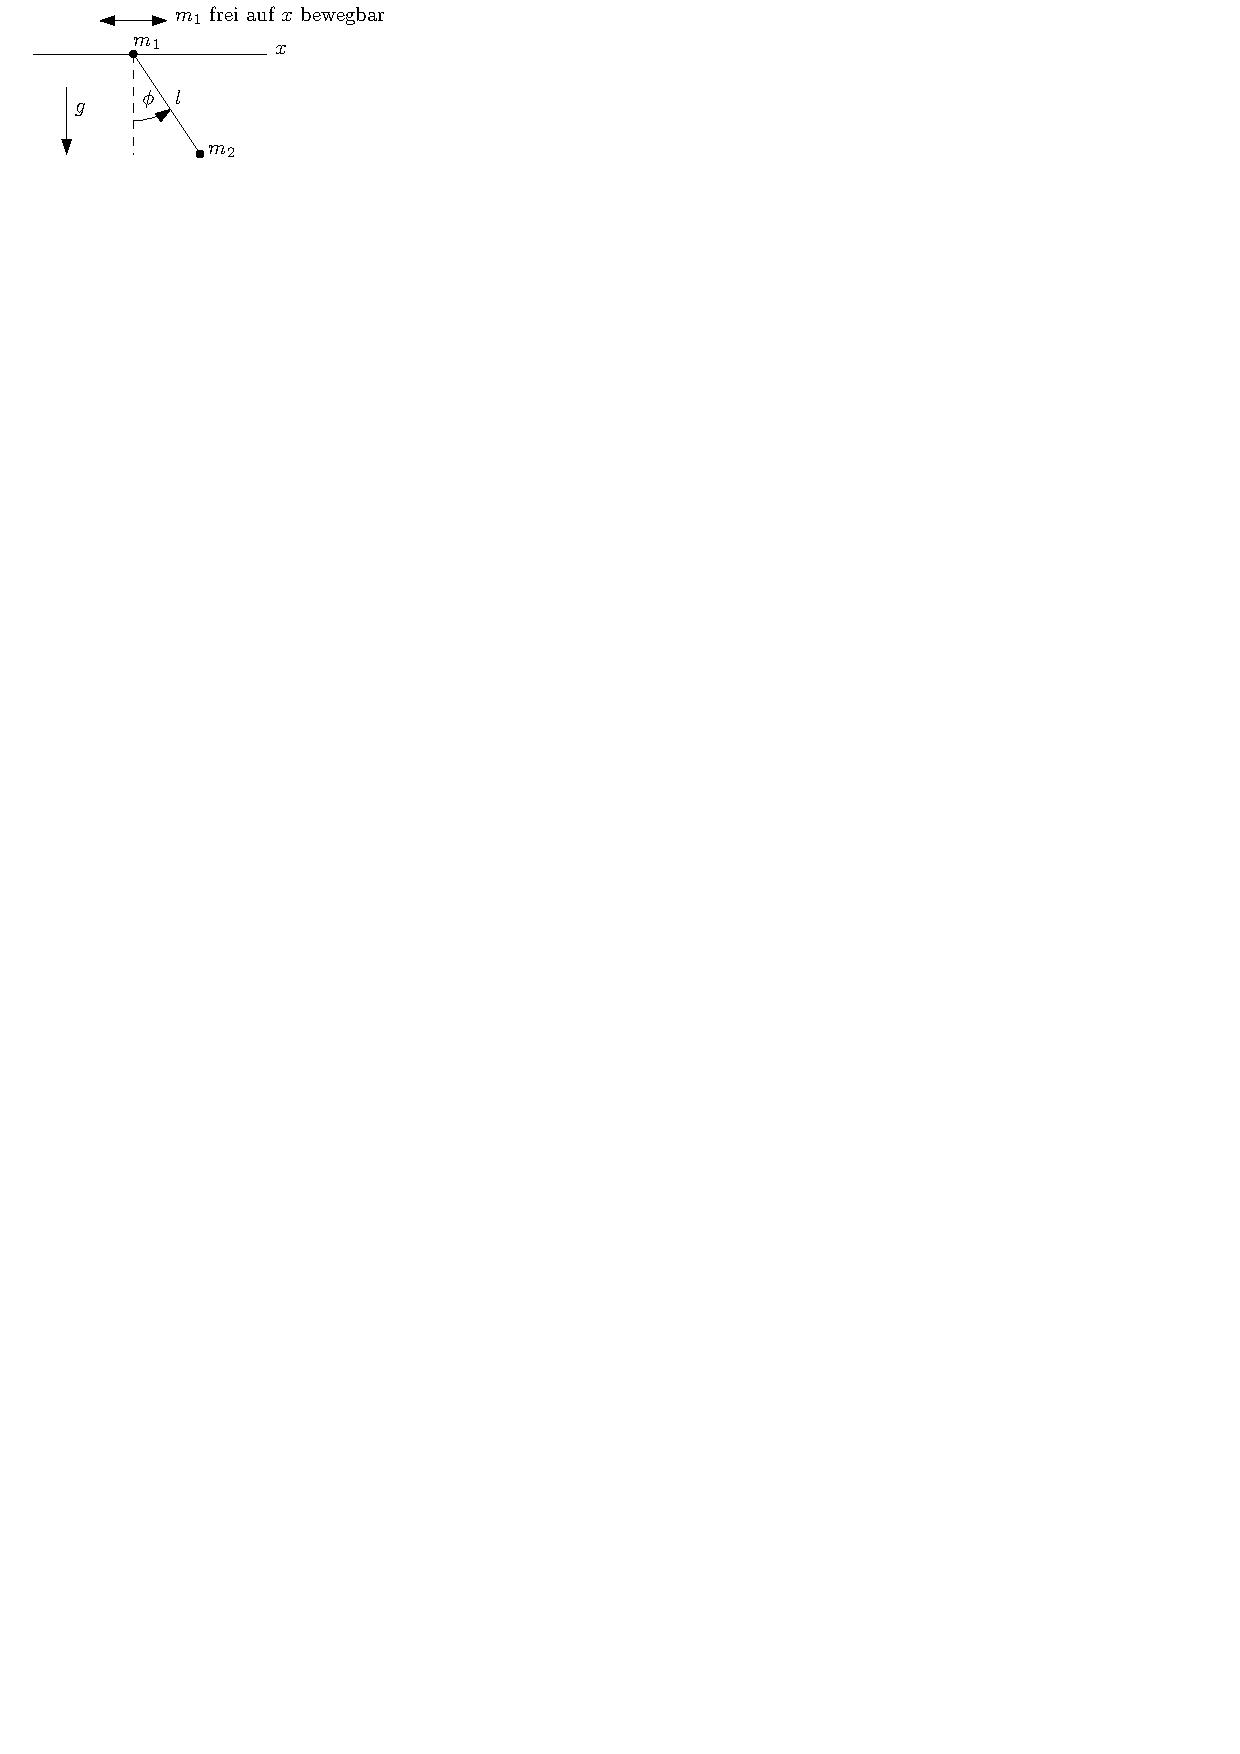
\includegraphics{figures/ch1/schwingendehantel}
		\caption{Schwingende Hantel, die an $x$-Achse aufgehängt ist. Massepunkt $m_1$ kann sich frei auf der $x$-Achse bewegen.}
		\label{fig:ch1_schwingendehantel}	
	\end{figure}

	Die Masse $m_1$ ist frei in $x$-Richtung beweglich und an der Masse $m_2$ zieht die Gravitationskraft.
	Es gibt die folgenden 4 holonom-skleronomen Zwangsbedingungen:
	\begin{align*}
	z_1 = z_2 &= 0, \\
	y_1 &= 0, \\
	(x_1 - x_2)^2 + y_2^2 - l^2 &= 0 \text{.}
	\end{align*}
	ALso gibt es im System $s = 6 - 4$ Freiheitsgrade.
	Als generalisierte Koordinaten kann man zum Beispiel $q_1 = x$ und $q_2 = \phi$ (der Winkel zwischen Lot und Hantelstange) wählen. Damit sind die Koordinaten und Geschwindigkeiten:
	\begin{align*}
	x_1 &= q_1 & x_2 &= q_1 + l \sin q_2\\
	y_1 &= 0 & y_2 &= l \cos q_2\\
	z_1 &= 0 & z_2 &= 0\\
	\dot{x}_1 &= \dot{q}_1 & \dot{x}_2 &= \dot{q}_1 + \dot{q}_2 l \cos q_2\\
	&&\dot{y}_2 &= - l \dot{q}_2 \sin q_2
	\end{align*}
	
	Schließlich folgt für die kinetische Energie:
	\begin{align*}
	T & = \frac12 m_1 \vecdotnumsq{r}{1} + \frac12 m_2 \vecdotnumsq{r}{2} \\
	&= \frac12 m_1 (\dot{x}_1^2 + \dot{y}_1^2 + \dot{z}_1^2) + \frac12 m_2 (\dot{x}_2^2 + \dot{y}_2^2 + \dot{z}_2^2) \\
	&= \frac12 m_1 \dot{q}_1^2 + \frac12 m_2 ( (\dot{q}_1 + \dot{q}_2 l \cos q_2)^2 + l^2 \dot{q}_2^2 \sin^2 q_2) \\
	&= \frac12 (m_1 + m_2) \dot{q}_1^2 + \frac12 m_2 (2 \dot{q}_1 \dot{q}_2 l \cos q_2 + \dot{q}_2^2 l^2) 
	\text{.}
	\end{align*}
	
	Mit dem Potential $V = 0 - m_2 g \cos(q_2)$ folgt die Lagrange-Funktion:
	\begin{align*}
		L &= T - V \\
		&= \frac12 (m_1 + m_2) \dot{q}_1^2 + \frac12 m_2 (l^2 \dot{q}_2^2 + 2 l \dot{q}_1 \dot{q}_2 \cos q_2) + m_2 g l \cos q_2
		\text{.}
	\end{align*}
	
	\textbf{Interessante Beobachtung}: $L$ hängt nicht von $q_1$ ab (nur von $\dot{q}_1$):
	\[
	\dd t \ffpartial{L}{\dot{q}_1} - \underbrace{\ffpartial{L}{q_1}}_{= 0} = 0
	\quad \text{und damit} \quad 	
	\ffpartial{L}{\dot{q}_1} = \text{konstant}
	\text{.}
	\]
\end{beispiel*}

\begin{definition*}[Zyklische Koordinate]\label{zyklische_koordinate}
	Ein Koordinate $q_j$ ist genau dann zyklisch falls gilt
	\[
		\ffpartial{L}{q_j} = 0 \Leftrightarrow \ffpartial{L}{\dot{q}_j} = \text{konstant} \equiv p_j
	\]
	mit dem verallgemeinerten Impuls 
	\[
		p_j = \ffpartial{L}{\dot{q_j}}
		\text{.}
	\]
	Zyklische Koordinaten führen automatisch zu einem \textit{Erhaltungssatz}. Deswegen sollten möglichst viele generalisierte Koordinaten zyklisch sein.
\end{definition*}

\begin{beispiel*}[Schwingende Hantel \textendash~Fortsetzung]
	\begin{align*}
		p_1 &= \ffpartial{L}{\dot{q}_1} = (m_1 + m_2)\dot{q}_1 + m_2 l \dot{q}_2 \cos(q_2) = \const = c'\\
		\Rightarrow \dot{q}_1 &= - \frac{m_2 l}{m_1 + m_2} \dot{q}_2 \cos(q_2) + c\\
		\overset{\text{Integration}}{\Rightarrow} q_1(t) &= ct - \frac{m_2 l}{m_1 + m_2} \sin (q_2(t))
	\end{align*}
	Die Anfangsbedingungen:
	\begin{align*}
		q_1(t = 0) &= q_2(t = 0) = 0 \\
		\dot{q}_2(t=0) &= \omega_0 \\
		\dot{q}_1(t=0) &= - \frac{m_2 l}{m_1 + m_2} \omega_0 \\
	\end{align*}
	Mit $q_1(t)$ von oben folgt $c = 0$ und wir bekommen $q_1(t) = - \frac{m_2 l}{m_1 + m_2} \sin q_2(t)$. Nun führen wir die Rücktransformation durch:

	\begin{align*}
		x_1(t) &= - \frac{m_2 l}{m_1 + m_2} \sin \phi(t), \\
		y_1(t) &= 0, \\
		x_2(t) &= - \frac{m_2 l}{m_1 + m_2} \sin \phi(t) + l \sin \phi(t) = \frac{m_1}{m_1 + m_2} l \sin \phi(t), \\
		y_2(t) &= l \cos \phi(t), \\
	\end{align*}
	wobei wir bei $x_2(t)$ die Identität $l = \frac{m_1 + m_2}{m_1 + m_2} l$ genutzt haben. Nur verwendet man die 3. Zwangsbedingung vom Anfang
	\begin{align*}
	(x_1 - x_2)^2 + y_2^2 - l^2 &= 0\\
	\Leftrightarrow \frac{(x_1 - x_2)^2}{l^2} + \frac{y_2^2}{l^2} &= 1\\ 
	\Leftrightarrow \frac{x_2^2(t)}{(\frac{m_1 l}{m_1 + m_2})^2} + \frac{y_2^2(t)}{l^2} &= 1
	\end{align*}
	Das beschreibt eine Ellipse mit den Halbachsen $\frac{m_1}{m_1 + m_2}l < l \text{~und~} l$.
	Dazu die $q_2$-Lagrange-Gleichung
	\begin{align*}
	\ffpartial{L}{\dot{q}_2} &= m_2 (l^2 \dot{q}_2 + l \dot{q}_1 \cos q_2)\\
	\dd t \ffpartial{L}{\dot{q}_2} &= m_2 (l^2 \ddot{q}_2 + l \ddot{q}_1 \cos q_2 - l \dot{q}_1 \dot{q}_2 \sin q_2)\\
	\ffpartial{L}{q_2} &= m_2 (- l \dot{q}_1 \dot{q}_2 \sin q_2 - g l \sin q_2)\\
	0 &= m_2 (l^2 \ddot{q}_2 + l \ddot{q}_1 \cos q_2 + g l \sin q_2)\\
	\intertext{Jetzt $\ddot{q}_1$ von oben (per Differentiation)}
	\ddot{q}_1 &= - \frac{m_2 l}{m_1 + m_2} (\ddot{q}_2 \cos q_2 - \dot{q}_2^2 \sin q_2)
	\end{align*}
	Damit erhält man die $q_2$-Gleichung
	\[
		l^2 \ddot{q}_2 - \frac{m_2 l^2}{m_1 + m_2}(\ddot{q_2} \cos q_2 - \dot{q}_2^2 \sin q_2) \cos q_2 + g l \sin q_2 = 0
		\text{.}
	\]
	Das ist eine nichtlineare \Dgl{} 2. Ordnung für $q_2(t) = \phi(t)$, die man vermutlich nicht per Hand lösen kann (aber numerisch). Man kann das Lösen aber durch weitere Annahmen über das System vereinfachen, zum Beispiel durch die Beschränkung auf kleine $\phi$:
	\[
		\phi(t) = \frac{\omega_0}{\omega} \sin \omega t \text{~und~} \omega = \sqrt{\frac{g}{l} \frac{m_1 + m_2}{m_1}}
		\text{.}
	\]
\end{beispiel*}


\subsubsection{Rezept für holonome Zwangsbedingungen}

Für die häufigsten Fälle mit \textbf{holonomen} Zwangsbedingungen und \textbf{konservativen} Kräften gibt es ein Rezept:
\begin{enumerate}
\item Zwangsbedingungen formulieren
\item Generalisierte Koordinaten festlegen
\item Lagrange-Funktion hinschreiben (mit generalisierten Koordinaten und Geschwindigkeiten)
\item Lagrange-Funktion ableiten und wenn möglich lösen
\item Eventuell Rücktransformation auf gewöhnliche (anschauliche) Koordinaten
\end{enumerate}

\subsubsection{Nicht-holonome Systeme}
Bei holonomen Systemen gibt es $S = 3N - p$ unabhängige generalisierte Koordinaten. Diese sind bei nicht-holonomen Systemen nicht mehr unabhängig.

Falls die nicht-holonomen Zwangsbedingungen in differentieller Form vorliegen (also als Differentialgleichung) gibt es ein Lösungsverfahren über die Methode der sogenannten Lagrange-Multiplikatoren, welche im folgenden erläutert werden.

Es gibt $\bar{p}$ Zwangsbedingungen, davon $p \leq \bar{p}$ nicht-holonom: 
\[
	i = 1, \dots, p: 
	\quad 
	\left( \sum_{m=1}^{3N} f_{im}(x_1, \dots, x_{3N}, t) \d x_m \right) + f_{it}(x_1, \dots, x_{3N}, t) \d t = 0
\]
mit $j = 3N - (\bar{p} - p)$ generalisierten Koordinaten.

Die konkreten Koordinaten hängen von den generalisierten ab: $\vec{r}_i = \vec{r}_i(\vardots{q}{j}, t)$, aber nicht alle $q_j$ sind unabhängig voneinander, wie anfangs schon erwähnt.

Damit gilt für nicht-holonome Bedingungen in $q_j$, wobei im Folgenden immer $i = 1, \dots, p$ ist:
\[
	\sum_{i=1}^j a_{im}(q_1, \dots, q_j, t) \d q_m + b_{it}(q_t, \dots, q_j, t) \d t = 0
	\text{.}
\]

Für virtuelle Verrückungen, bei denen $\delta t = 0$ gilt, ist die Gleichung wie folgt:
\[
	\sum_{m=1}^j a_{im} \delta q_m = 0
	\text{.}
\]

Nun werden die Lagrange-Multiplikatoren $\lambda_i = \lambda_i(t)$ eingeführt (nicht von $q_i$ abhängig, sondern nur von der Zeit):
\[
	\sum_{i=1}^{p} \lambda_i \sum_{m=1}^j a_{im} \delta q_m = 0
	\text{.}
\]
Bei konservativen Systemen (siehe oben) gilt mit dem Prinzip von d'Alembert:
\[
	\sum_{m=1}^j \left( \ffpartial{L}{q_m} - \dd t \ffpartial{L}{\dot{q}_m} \right) \delta q_m = 0
\]

Wobei diese Gleichung nur als Summe gültig ist, da die $\delta q_m$ nicht mehr unabhängig voneinander sind. Zusammengefasst folgt
\[
	\sum_{m=1}^j \left( \ffpartial{L}{q_m} - \dd t \ffpartial{L}{\dot{q}_m} + \sum_{i=1}^p \lambda_i a_{im} \right) \delta q_m = 0
	\text{.}
\]

Nur ein Teil der generalisierten Koordinaten ist, wie schon oft erwähnt, unabhängig voneinander: $m = 1, \dots, j - p$ sind unabhängig und $m = j - p + 1, \dots j$ (genau $p$ Bedingungen) sind abhängig, die Wahl der $q_m$ findet dementsprechend statt.

Wähle für die letzten $p$ Gleichungen die bisher nicht bestimmten $\lambda_i$ so, dass
\[
	m = j-p+1, \dots, j: 
	\quad 
	\ffpartial{L}{q_m} - \dd t \ffpartial{L}{\dot{q}_m} + \sum_{i=1}^p \lambda_i a_{im} = 0
	\text{.}
\]
Das geht, da es $p$ Gleichungen und genauso viele $\lambda_i$'s gibt. Damit hat man nur noch Gleichungen mit unabhängigen $q_m$, also
\[
	\sum^{j - p}_{m = 1} \left( \ffpartial{L}{q_m} - \dd t \ffpartial{L}{\dot{q}_m} + \sum^p_{i = 1} \lambda_i a_{im} \right) \delta_{q_m} = 0
	\text{.}
\]
Hier kann man die $\delta_{q_m}$ unabhängig variieren, also jeder Summand $=0$. Daraus entstehen Lagrange-Gleichungen 1. Art entstehen für alle $m$:
\[
	m = 1, \dots, j:
	\quad
	\dd t \ffpartial{L}{\dot{q}_m} - \ffpartial{L}{q_m} = \sum_{i=1}^p \lambda_i a_{im}
	\text{.}
\]
Hierbei gilt noch $\sum_{m=1}^j a_{im} \dot{q}_m + b_{it} = 0$ für $i = 1, \dots, p$. Damit hat man $j + p$ Gleichungen für $j$ generalisierte Koordinaten und $p$ Multiplikatoren $\lambda_i$.

Ein Vergleich mit den generalisierten Kräften zeigt $\bar{Q}_m = \sum_{i=1}^{p} \lambda_i a_{im}$.
Nun hat man generalisierte Zwangskräfte ($\sum_{m=1}^j \bar{Q}_m \delta q_m = 0$) was den $\lambda_i$ entspricht.
Dieses Wissen ist auch ein Gewinn für Systeme mit holonomen Zwangsbedingungen, denn die Kenntnis der Zwangskräfte ist nützlich für das Design des Systems.

\textbf{Anwendung auf holonome Systeme}: 
$f_i(\vardots{\vec{r}}{N}, t) = 0, i = 1, \dots, p$ in generalisierten Koordinaten $\bar{f}_i(\vardots{q}{j}, t) = 0$, daraus folgt das totale Differential 
\[
	\d \bar{f}_i = \sum_{m=1}^j \ffpartial{\bar{f}_i}{q_m} \d q_m + \ffpartial{\bar{f}_i}{t} \d t
\]
und damit ($\d \bar{f}_i = 0$ für $i = 1, \dots, p$)
\[
	a_{im} = \ffpartial{\bar{f}_i}{q_m}
	\quad \text{sowie} \quad
	b_{it} = \ffpartial{\bar{f}_i}{t}
	\text{.}
\]
Die Zwangskräfte in holonomen Systemen können nun mit Lagrange-Gleichungen 1. Art bestimmt werden.

\begin{beispiel*}[holonome Zwangsbedingungen mit Zwangskräften]
Es wird ein Pendel mit Winkel $\varphi$ zum Lot, der Länge $l$ und der Masse $m$ betrachtet (siehe Abbildung \ref{fig:ch1_fadenpendel}).
\begin{figure}
	\centering
	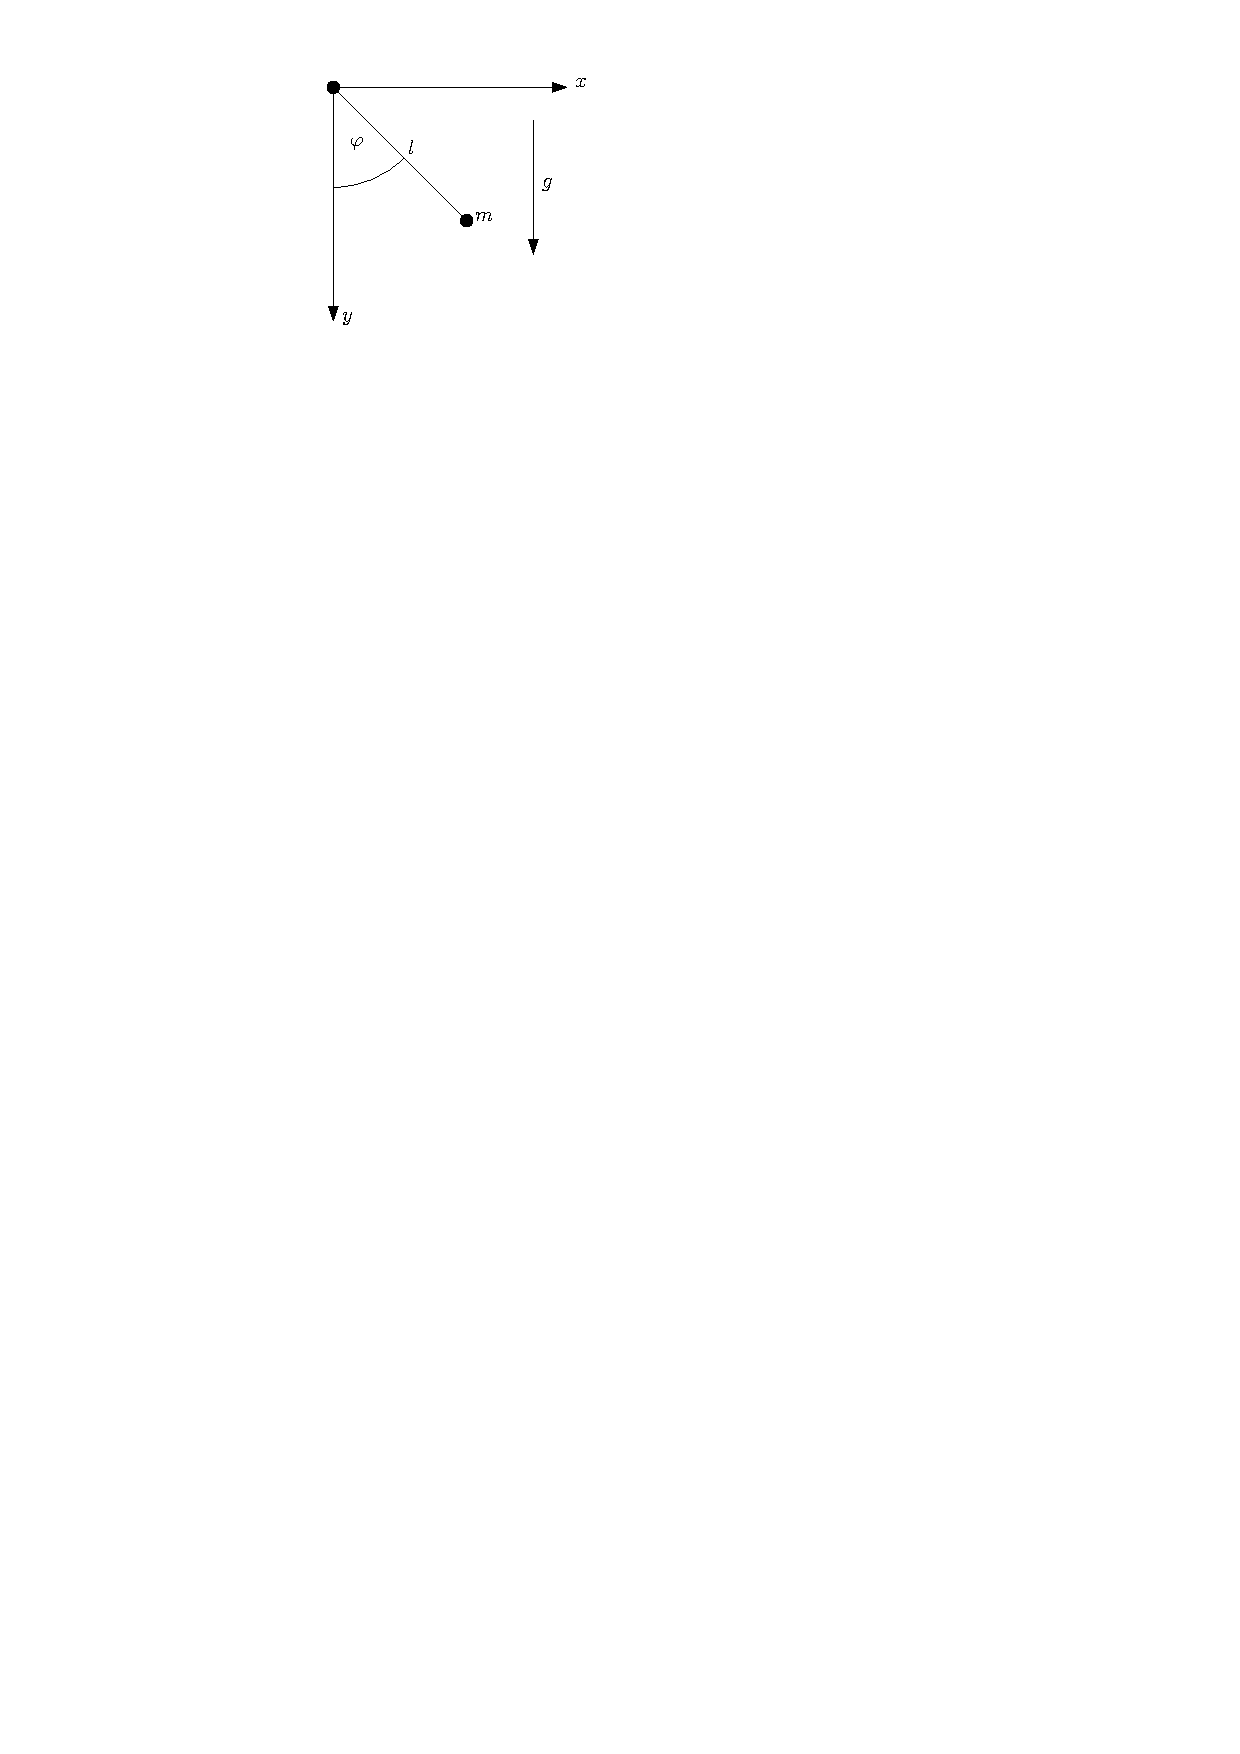
\includegraphics{figures/ch1/fadenpendel}
	\caption{Ein Fadenpendel der Masse $m$.}
	\label{fig:ch1_fadenpendel}
\end{figure}
Zunächst wird $r=l$ variabel gewählt. Die verallgemeinerten Koordinaten sind deswegen $\varphi$ und $r$.
\begin{align*}
x &= r \sin \varphi\\
y &= l - r \cos \varphi\\
f(x,y,t) &= r - l = 0 \text{~~~~ist die Zwangsbedingung}\\
V &= -mg y = -mg (l -r \cos \varphi)\\
T &= \frac12 m (\dot{x}^2 + \dot{y}^2)\\
\dot{x} &= \dot{r} \sin \varphi + r \dot{\varphi} \cos \varphi\\
\dot{y} &= - \dot{r} \cos \varphi + r \dot{\varphi} \sin \varphi\\
\dot{x}^2 + \dot{y}^2 &= \dot{r}^2 \sin^2 \varphi + 2 r \dot{r} \dot\varphi \sin \varphi \cos \varphi \\
&+ r^2 \dot{\varphi}^2 \cos^2 \varphi + \dot{r}^2 \cos^2 \varphi - 2 r \dot r \dot \varphi \sin \varphi \cos \varphi + r^2 \dot{\varphi}^2 \sin^2 \varphi \\
&= \dot{r}^2 + r^2 \dot{\varphi}^2\\
L &= T-V = \frac12 m (\dot{r}^2 + r^2 \dot{\varphi}^2) + mg(l - r \cos \varphi)\\
\ffpartial{L}{r} - \dd t \ffpartial{L}{\dot{r}} &= m r \dot{\varphi}^2 - mg \cos \varphi - \dd t m \dot{r} \\
&= -m (g \cos \varphi + \ddot{r} - r \dot{\varphi}^2)\\
\ffpartial{L}{\varphi} - \dd t \ffpartial{L}{\dot{\varphi}} &= mgr \sin \varphi - \dd t m r^2 \dot{q} \\
&= mgr \sin \varphi - 2mr\dot{r}\dot{\varphi} - mr^2 \ddot{\varphi}\\
\end{align*}
Zwangsbedingung $r-l = 0 = \bar{f}(r, \varphi, t)$\\
$\ffpartial{f}{r} = 1$ alle anderen partiellen Ableitungen $= 0$\\
\conseq $\lambda_r = \bar{Q}_r$ ist Zwangskraft in $r$-Richtung

Daraus folgen die drei Gleichungen:
\begin{itemize}
	\item \textbf{$r$-Gleichung}: $\lambda = m \ddot{r} + mg \cos \varphi - m r \dot{\varphi}^2$,
	\item \textbf{$\varphi$-Gleichung}: $\ddot{\varphi} + \frac{2 \dot{r}}{r} \dot{\varphi} + \frac{g}{r} \sin \varphi = 0$ und
	\item \textbf{$l$-Gleichung}: $r = l \rightarrow \dot{r} = \ddot{r} = 0$.
\end{itemize}
Randbemerkung: $\lambda = -m(l \dot{\varphi}^2 - g \cos \varphi)$ ist hier die Fadenspannung.

Das ganze kann man vereinfachen wenn man $\dot{r} = 0$ und $\sin \varphi \approx \varphi$ annimmt (letzteres gilt für kleine $\varphi$). Damit gilt dann folgendes ($\ddot{\vp} + \frac{g}{l} \vp = 0$)
$$\varphi(t) = \varphi_0 \sin \sqrt{\frac{g}{l}} t$$
\end{beispiel*}

\subsection{Das Hamiltonsche Prinzip}	
Wir zeigen, dass die Lagrange-Gleichungen nicht nur aus dem differentiellen Prinzip von d'Alembert folgen: gerade hatten wir momentane virtuelle Verrückungen betrachtet.
\textbf{Dagegen Hamilton}: \textbf{Integralprinzip}\\
Das ist die Variation der gesamten Bahn bei festen Endpunkten.
Dazu betrachten wir Bahnen $\vec{q}(t)$ im Konfigurationsraum
$$\vec{q}(t) = (q_1(t), \dots, q_s(t))$$
ein $\vec{q}(t)$ beschreibt einen Zustand des gesamten Systems. Für gegebene $\vec{q}(t)$ und $\dot{\vec{q}}(t)$ wird die Lagrange-Funktion eine Funktion der Zeit 
$$L(\vec{q}(t), \dotvec{q}(t), t) = \tilde{L}(t)$$

\begin{definition*}[Wirkungsfunktional]
$$S\{\vec{q}(t)\} = \int_{t_1}^{t_2} \tilde{L}(t) \d t$$
Die Dimension hiervon ist "`Wirkung"' \conseq Energie:
$S$ hängt von $\vec{q}(t)$ und $t_1, t_2$ ab. 
Funktion $\vec{q}(t) \xrightarrow{\text{Abbildung}} S \{ \vec{q}(t) \}$ im allgemeinen Funktional.

Wir betrachten Scharen $\vec{q}(t)$ mit den gleichen Endpunkten $\vec{q}(t_1)$ und $\vec{q}(t_2)$. Virtuelle Verrückungen müssen verschwinden.	
\end{definition*}


Beim Hamiltonschen Prinzip wird nun die Bahn des Systems betrachtet und wir wollen eine extremale Bahn finden.

~\\
\begin{definition*}[Hamiltonsches Prinzip]
Die Systembewegung erfolgt so, dass $S\{\vec{q}(t)\}$ für die richtige Trajektorie extremal wird, d.h. dass die Variation bezüglich der tatsächlichen Bahn verschwindet.
$$\delta S = \delta \int_{t_1}^{t_2} L(\vec{q}(t), \dotvec{q}(t), t) \d t \overset{!}{=} 0$$
\end{definition*}

\begin{bemerkung*}
	Die Gleichung $\delta S = 0$ enthält auf elegante Weise die gesamte klassische Mechanik. Das Prinzip (der Minimierung der Trajektorie) wird auch jenseits der Mechanik verwendet\footnote{Zum Beispiel in der Teilchenphysik, der geometrischen Optik (Fermatsches Prinzip, dabei bewegt sich Licht auf einer Bahn, so dass die benötigte Zeit minimal ist. Damit können die Brechungsindizes gefunden werden.)}. Es ist natürlich koordinatenunabhängig.
\end{bemerkung*}

\begin{bemerkung*}
	Das Hamiltonsche Prinzip wird auch jenseits der klassischen Mechanik verwendet. Beispielsweise in der Teilchenphysik (Quantenfeldtheorie) oder in der Optik.
\end{bemerkung*}

\subsubsection{Äquivalenz zum Prinzip von d'Alembert}
\begin{align*}
\sum_{i=1}^N (m_i \ddotvec{r}_i - \vec{K}_i) \delta \vec{r_i} &= 0\\
\intertext{Integration über die Zeit}
\int_{t_1}^{t_2} (\sum_{i=1}^N (m_i \ddotvec{r}_i - \vec{K}_i) \delta \vec{r_i}) \d t &= 0
\intertext{mit $\ddotvec{r}_i \delta \vec{r}_i = \dd t (\dotvec{r}_i \cdot \delta \vec{r}_i) - \dotvec{r}_i \cdot \delta \dotvec{r}_i = \dd t (\dotvec{r}_i \cdot \delta \vec{r}_i) - \frac12 \delta \dot{(\vec{\hspace{-1em}r\hspace{1em}}_i^2)}$}
\int_{t_1}^{t_2} (\sum_{i=1}^N (\dd t (m_i \dotvec{r}_i \cdot \vec{r}_i) - \frac12 m_i \delta (\dotvec{r}_i^2) - \vec{K}_i \cdot \delta \vec{r}_i) \d t &= 0
\intertext{Integration}
\int_{t_1}^{t_2} \sum_{i=1}^N \dd t (m_i \dotvec{r}_i \cdot \delta \vec{r}_i) \d t
=  \left. \sum_{i=1}^N m_i \dotvec{r}_i \cdot \delta \vec{r}_i \right|_{t_1}^{t_2} &= 0\\
\intertext{Keine Variation an den Endpunkten}
\Rightarrow \int_{t_1}^{t_2} \sum_{i=1}^N [ \delta (\frac{m_i}{2} \dotvec{r}_i^2 ) + \vec{K}_i \cdot \delta \vec{r}_i ] \d t &= 0
\intertext{mit $\vec{r}_i = \vec{r}_i(q_1, \dots, q_s, t)$, $i = 1, \dots, N$ findet man die generalisierte Kraft und das konservative Potential mit holonomen Zwangsbedigungen.}
\sum_{i=1}^N \vec{K}_i \delta \vec{r}_i = \sum_{j=1}^s Q_j \delta q_j = \sum_{j=1}^{s} - \ffpartial{V}{q_j} \delta q_j &= - \delta V
\intertext{Daraus folgt dann zusammen genommen die Äquivalenz des Prinzips von d'Alembert und dem Hamiltonschen}
0 = \int_{t_1}^{t_2} \delta (T-V) \d t = \delta \int_{t_1}^{t_2} (T-V) \d t = \delta \int_{t_1}^{t_2} L \d t &= 0
\end{align*}

Bewegungsgleichungen? \conseq Variationsrechnung.
Finden der Kurve $\vec{q}(t)$, die $S\{\vec{q}(t)\}$ extremal macht.

\subsubsection{Elemente der Variationsrechnung}

\begin{definition*}[Euler-Gleichung]
	Sie ist aufgebaut wie die Lagrange-Gleichung, gilt aber ganz allgemein für Variationsprobleme.
	$$ \ffpartial{f}{y} - \dd x \ffpartial{f}{y'} = 0$$
\end{definition*}~\\
Zunächst ein eindimensionales Problem.
\paragraph{Problem} Finde eine Kurve $y(x)$ für die ein bestimmtes Funktional extremal wird. Zum Beispiel "`eine kürzeste Verbindung"', beispielsweise auf einer krummen Fläche (Geodäte) wie einer Seifenhaut.
Die verschiedenen möglichen Verbindungen bilden eine Schar $f(x, y, y')$ von $y(x)$ mit festen Endpunkten. Es wird angenommen, dass $f$ differenzierbar in allen Variablen ist. Im folgenden gilt weiterhin $y' = \ddd{y}{x}$.
Wir bilden das Funktional
\begin{align*}
J\{y(x)\} &= \int_{x_1}^{x_2} f(x, y, y') \d x = \int_{x_1}^{x_2} \tilde{f}(x) \d x
\end{align*}
Das Problem kann nun wie folgt ausgedrückt werden: Für welches $y(x)$ wird $J\{y(x)\}$ extremal?\\
Dies ist ähnlich zu einer einfachen Extremwertaufgabe, wenn die Schar $y(x)$ durch den Parameter $\alpha$ parametrisiert werden kann. Dies kann zum Beispiel so geschehen, dass
\begin{align*}
y_{\alpha = 0}(x) &= y_0(x)
\intertext{die extremale und damit gesuchte Bahn wird. Damit kann man jetzt $y_\alpha$ aufteilen}
y_\alpha(x) &= y_0(x) + \gamma_\alpha(x)
\intertext{$\gamma_\alpha(x)$ ist hierbei eine fast beliebige, differenzierbare Funktion, welche an den Endpunkten für alle $\alpha$ verschwindet, also 0 wird. Nach dem, wie $\gamma_\alpha$ konstruiert wurde gilt auch}
\gamma_{\alpha = 0}(x) &= 0~~~\forall x
\intertext{Man kann $\gamma_\alpha$ auch anders angeben: $\gamma_\alpha(x) = \alpha \eta(x), ~~~ \eta(x_1) = \eta(x_2) = 0$. $x$ wird festgehalten und dann eine Taylorreihe mit $\alpha = 0$ wie folgt entwickelt}
\gamma_\alpha(x) &= \alpha (\ffpartial{\gamma_\alpha(x)}{\alpha})_{\alpha = 0} + \frac{\alpha^2}{2} (\frac{\partial^2 \gamma_\alpha(x)}{\partial \alpha^2})_{\alpha = 0} + \dots
\intertext{Oder wieder anders}
\gamma_\alpha(x) &= y_0(x) + \alpha(\ffpartial{y_\alpha}{\alpha})_{\alpha = 0} + \dots
\end{align*}

$y_\alpha(x)$ wird nun in der Nähe (besser gesagt in der $\epsilon$-Umgebung) von $\alpha = 0$ variiert. Daraus folgt, dass $\alpha \rightarrow \d \alpha$.
Und damit $\delta y = y_{\d \alpha} - y_0(x) = \d \alpha (\ffpartial{y_\alpha(x)}{\alpha})_{\alpha = 0}$.
Wird nun $\delta y$ bei festem $x$ betrachtet (vgl. virtuelle Verrückungen bei fester Zeit t. ($\delta t = 0$)) kommt man zu einer Variation des Funktionals $J\{y(x)\}$
\begin{align*}
\delta J &= J \{ y_{\d \alpha}(x) \} - J\{ y_0(x)\} = (\ddd{J(x)}{\alpha})_{\alpha = 0} \d \alpha\\
&= \int_{x_1}^{x_2} (f(x, y_{\d \alpha}, y'_{\d \alpha}) - f(x, y_0, y'_0)) \d x
\end{align*}
Jetzt ist die Extremalbedingung offensichtlich: Es muss für beliebige $\gamma_{\alpha}(x)$ gelten
$$(\ddd{J(\alpha)}{\alpha})_{\alpha = 0} = 0$$
Damit ist $y_0(x)$ eingesetzt ist die gesuchte Bahn. Es ist eine stationäre Bahn genau dann, wenn $\delta J \overset{!}{=} 0$.
Durch einfaches Umformen folgt damit
\begin{align*}
(\ddd{J(\alpha)}{\alpha}) &= \int_{x_1}^{x_2} \d x (\ffpartial{f}{y} \ffpartial{y}{\alpha} + \ffpartial{f}{y'} \ffpartial{y'}{\alpha} + \ffpartial{f}{x} \ffpartial{x}{\alpha})
\intertext{mit der Identität $\int_{x_1}^{x_2} \d x \ffpartial{f}{y'} \ffpartial{y'}{\alpha} = \int_{x_1}^{x_2} \d x \ffpartial{f}{y'} \dd x \ffpartial{y}{\alpha}$, $\ffpartial{y'}{\alpha} = \fpartial{\alpha} \ddd{y}{x} = \dd x \ffpartial{y}{\alpha}$ und partieller Integration folgt}
&= \underbrace{\left. \ffpartial{f}{y'} \ffpartial{y}{\alpha} \right|_{x_1}^{x_2}}_{\hspace{-10em}=0, \text{~da keine Variation an den Endpunkten.\hspace{-10em}}} - \int_{x_1}^{x_2} \d x (\dd x \ffpartial{f}{y'}) \ffpartial{y}{\alpha}\\
\dd \alpha J(x) &= \int_{x_1}^{x_2} \d x (\ffpartial{f}{y} - \dd x \ffpartial{f}{y'}) \ffpartial{y}{\alpha}\\
\delta J &= \int_{x_1}^{x_2} \d x (\ffpartial{f}{y} - \dd x \ffpartial{f}{y'}) \delta y
\end{align*}
$\delta J \overset{!}{=} 0$ für beliebige $\delta y$ damit verschwindet der Integrand. Daraus folgt wieder die Eulersche Gleichung
$$\ffpartial{f}{y} - \dd x \ffpartial{f}{y'} = 0$$
Und damit eine Differentialgleichung 2. Ordnung für das gesuchte $y(x)$. (vgl. Lagrange-Gleichung 2. Art)

\begin{beispiel*}[Kürzeste Verbindung zweier Punkte in der Ebene]~\\
	Welches Funktional? (Infinitesimale Länge $\d s = \sqrt{\d x^2 + \d y^2}$) Gesucht ist $\int_{p_1}^{p_2} \d s = J$\\
	$$J = \int_{p_1}^{p_2} \d s = \int_{x_1}^{x_2} \sqrt{\d x^2 + \d y^2} = \int_{x_1}^{x_2} \sqrt{1 + (\ddd{y}{x})^2} \d x = \int_{x_1}^{x_2} \sqrt{1 + {y'}^2} \d x$$
	$\delta J = 0$ führt zur extremalen Bahn $y(x)$. 
	$$ f(x, y, y') = \sqrt{1 + {y'}^2}$$
	Nun verwenden wir die Euler-Gleichung: $\ffpartial{f}{y} = 0$; $\ffpartial{f}{y'} = \frac{y'}{\sqrt{1 + {y'}^2}}$ und damit folgt
	$$\dd x \frac{y'}{\sqrt{1 + {y'}^2}} = 0$$
	oder anders gesagt
	$$\frac{y'}{\sqrt{1 + {y'}^2}} = \text{konstant} = c \qquad \Rightarrow \qquad {y'}^2 = c^2 ( 1 + {y'}^2)$$
	Zusammenfassend folgt damit mit ${y'}^2(1 - c^2) = 1$, dass $y'$ konstant ist
	und damit schlussendlich auch die Lösung des Problems
	$$y(x) = a x + b$$
	$a$, $b$ werden über die Anfangsbedingungen$(x_1, y_1)$ und $(x_2, y_2)$ festgelegt.
\end{beispiel*}

\begin{beispiel*}[Minimale Rotationsfläche]~\\
Die Punkte $(x_1,y_1),(x_2,y_2)$ rotieren um die $y$-Achse. Gesucht ist die Kurve zwischen ihnen, welche die Rotationsfläche minimiert. (Seifenblasen-Verhalten.)
\textit{Es wird im Grunde genommen wie beim letzten Beispiel vorgegangen.} Die Minimalfläche ist
\begin{align*}
J &= \int \d A = \int 2 \pi x \d s
\intertext{mit $\d s = \sqrt{\d x^2 + \d y^2} = \sqrt{1 + (\ddd{y}{x})^2} \d x = \sqrt{1 + {y'}^2} \d x$ folgt}
&= 2 \pi \int_{x_1}^{x_2} x \sqrt{1 + {y'}^2} \d x
\end{align*}
Wenn $\delta J = 0$ gilt, ist $J$ die extremale Fläche, d.h. die minimalgroße Fläche.
Es wird nun die Funktion, besser gesagt die Variation, $f$ definiert 
\begin{align*}
f(x,y,y') &= x \sqrt{1 + {y'}^2} & \text{~\textit{mit }}y' = \ddd{y}{x}\\
\ffpartial{f}{y} &= 0 & \ffpartial{f}{y'} = \frac{x y'}{\sqrt{1 + {y'}^2}}\\
\xRightarrow[]{\text{Eulergleichung}} \dd x \frac{x y'}{\sqrt{1 + {y'}^2}} &= 0\\
\frac{x y'}{\sqrt{1 + {y'}^2}} &= \text{konstant} = a\\
\ddd{y}{x} &= y' = \frac{a}{\sqrt{x^2 - a^2}}\\
y(x) &= a \arcosh (\frac{x}{a}) + b & \text{~\textit{oder }} x(y) = a \cosh (\frac{y - b}{a})
\end{align*}
$a$, $b$ können wieder mithilfe der Anfangsbedingungen $(x_1, y_1)$ und $(x_2, y_2)$ gefunden werden.\\
Ein Hinweis am Rande: Die Kurve, welche durch den Kosinus Hyperbolicus beschrieben wird, wird auch Kettenlinie\footnote{\href{https://de.wikipedia.org/wiki/Kettenlinie_\%28Mathematik\%29}{Wikipedia}} genannt.
\end{beispiel*}

\subsubsection{Verallgemeinerung des Variationsproblems auf mehrere Variablen}
\textit{\dots und damit die Euler-Gleichung natürlich auch.}\\
Das betrachtete $y$ wird nun als Vektor $\vec{y}(x) = (y_1(x), \dots, y_s(x))$ geschrieben und ganz analog gilt
$$\delta J = \int_{x_1}^{x_2} \d x \sum_{i=1}^{s} (\ffpartial{f}{y_i} - \dd x \ffpartial{f}{y'_i}) \delta y_i = 0$$
Hierbei sind $\delta y_i$ die unabhängigen Freiheitsgrade. Offensichtlich gibt es eine Gleichung pro Freiheitsgrad
\begin{align*}
\ffpartial{f}{y_i} - \dd x \ffpartial{f}{y'_i} &= 0, i = 1, \dots, s
\intertext{Dies stellt in etwa die Euler-Lagrange-Gleichungen dar. Nun kann man das Hamiltonsche Prinzip anwenden}
\delta \int L(t, \vec{q}, \dotvec{q}) \d t &\overset{!}{=} 0
\intertext{Es funktioniert also völlig analog. Damit bekommt man Lagrange-Gleichungen 2. Art}
\dd t \ffpartial{L}{\dot{q}_i} - \ffpartial{L}{q_i} &= 0
\end{align*}
\conseq \textbf{Hamiltonsches Prinzip}
Das Integralprinzip (Hamilton) und das differentielle Prinzip (d'Alembert) sind äquivalent. Beide führen auf die Lagrange-Gleichungen. 

\textit{Das Hamiltonsche Prinzip wird ausgiebig in der Quantenmechanik verwendet. Im folgenden wird weiter auf die Hamilton-Funktion eingegangen um als Ziel sich in die Quantenmechanik zu bewegen. Es werden im speziellen Eigenschaften der Hamilton-Funktion angegeben.}

\subsubsection{Erhaltungsgrößen}
\paragraph{Allgemeines System} Die allgemeinen Koordinaten $q_i$, $\dot{q}_i$ für $i = 1, \dots, s$ sind im Laufe der Zeit veränderlich, womit es $2S$ Funktionen der Zeit gibt. Einige von diesen sind jedoch konstant\footnote{Mathematisch ausgedrückt gilt dann $F_r = F_r(q_1, \dots, q_s, \dot{q}_1, \dots, \dot{q}_s, t) = \text{konstant}$.}, was nicht Zufall sein muss.\footnote{Es ist aus offensichtlichen das Ziel, dass möglichst viele Funktionen konstant sind. Denn wie man schon im Lagrange-Teil gesehen hat, wird damit die Komplexität des Problems reduziert.}
Diese konstanten Funktionen heißen auch \textbf{Integrale der Bewegung}.

\paragraph{Im Prinzip gilt} Bei $2S$ Integralen der Bewegung $C_i$ ist das Problem gelöst, weil $q_i = q_i(C_1, \dots, C_{2S}, t)$ und damit das Problem nicht mehr dynamisch ist. Die Lösung kann dann einfach abgelesen werden.

Einige Konstanten der Bewegung hängen mit den Grundeigenschaften von Raum und Zeit zusammen (siehe unten).

Allgemein gilt, dass, wie schon gesagt, möglichst viele Konstanten der Bewegung bestimmt werden sollten, bevor die Lösung angestrebt wird. Einige der möglichen Konstanten haben wir schon kennengelernt: Die Resultate zyklischer Koordinaten: $q_i$ sei zyklisch\footnote{vgl. \ref{zyklische_koordinate}}, damit gilt
$$p_j = \ffpartial{L}{\dot{q}_j} = \text{konstant}$$
Ein gutes Beispiel hierfür sind Zweikörperprobleme.

\begin{beispiel*}[Zweikörperproblem\footnote{\href{http://de.wikipedia.org/wiki/Zweik\%C3\%B6rperproblem}{Wikipedia}}\footnote{Konkrete Beispiele sind die Anziehung zwischen Protonen und Elektronen im Atom oder jener zwischen Sonne und Erde.}]~\\
Zwei Massepunkte $m_1$ und $m_2$ haben die Koordinaten $\vec{r}_1$ und $\vec{r}_2$ und die Relativkoordinate $\vec{r} = \vec{r}_i - \vec{r}_2$. Als Kraft herrscht nur das Potentialfeld\footnote{Nur abhängig von der relativen Position der Massepunkte. Beispiele hierfür sind das Gravitationsfeld oder das elektrische Feld}
\begin{align*}
V(\vec{r}_1, \vec{r}_2) &= V(| \vec{r}_1 - \vec{r}_2|) = V(r)\\
\text{Gesamtmasse~~~} M &= m_1 + m_2\\
\text{reduzierte Masse~~~} \mu &= \frac{m_1 m_2}{m_1 + m_2}\\
\text{Schwerpunkt~~~} R &= \frac{1}{M} (m_1 \vec{r}_1 + m_2 \vec{r}_2)\\
\text{Relativkoordinate~~~} \vec{r} &= \vec{r}_1 - \vec{r}_2 = r (\sin \vartheta \cos \varphi, \sin \vartheta \sin \varphi, \cos \vartheta)
\end{align*}~\\
\emph{Wir Erwarten}
\dots das sowohl die Bewegung des Schwerpunkts trivial, also gleichförmig, ist wie auch die Bewegung der reduzierten Masse $\mu$ im Schwerpunktsystem ist.\\~\\
Die generalisierten Koordinaten sind in unserem Beispiel
\begin{align*}
\vec{R} &= (q_1, q_2, q_3) \text{~mit~} r = q_4, \vartheta = q_5, \varphi = q_6
\intertext{Damit ist die Lagrange-Funktion in den generalisierten Koordinaten}
	L &= \frac{M}{2} (\dot{q}_1^2 + \dot{q}_2^2 + \dot{q}_3^2) \\~&- V(q_4) + \frac{\mu}{2} (\dot{q}_4^2 + q_4^2 \dot{q}_5^2 + q_4^2 \dot{q}_6^2 \sin^2 q_5)
	\intertext{Offensichtlich sind die Koordinaten $q_1, q_2, q_3, q_6$ zyklisch und $p_i = \ffpartial{L}{\dot{q}_i} = M \dot{q}_i$ für ($i =1, 2, 3$), also bleibt der \textit{Schwerpunktimpuls} erhalten.}
	\vec{p} &= M \dotvec{R} = \text{konstant}\\
	p_6 &= \ffpartial{L}{\dot{q}_6} = \mu q_4^2 \dot{q}_6 \sin^2 q_5 = \mu \dot{\varphi} r^2 \sin^2 \vartheta = L_r^{(Z)} = \text{konstant}
\end{align*}
Die $z$-Komponente des Relativdrehimpulses ist offensichtlich konstant\footnote{Vergleiche: Geworfenes Frisbee, dessen Drehachse relativ gesehen sich nicht verändert.\footnote{Tipp: Dies mit einer Tafelkreide zu probieren ist aufgrund des vergleichsweise geringen Impulses schlecht möglich.}}.
Wenn man nun versucht das Problem in den Kartesischen Koordinaten anzugehen, führt das zu folgender Lagrange-Funktion:
\begin{align*}
	L =& \frac{m_1}{2} (\dot{x}_1^2 + \dot{y}_1^2 + \dot{z}_1^2) + \frac12 m_2 (\dot{x}_2^2 + \dot{y}_2^2 + \dot{z}_2^2) \\
	&- V((x_1 - x_2)^2 + (y_1 - y_2)^2 + (z_1 - z_2)^2)
	\intertext{Auch hier sind die Erhaltungssätze gültig. Sie sind aber viel schwerer abzulesen.}
\end{align*}
\end{beispiel*}

\subsubsection{Homogenität in der Zeit}
Das bedeutet die Invarianz der Bewegung gegenüber Zeittranslationen\footnote{Das gleiche zu einem späteren Zeitpunkt starten.}\footnote{Der Informatiker kennt das auch als seiteneffektfreie Funktion.} bei gleichen Anfangsbedingungen.
\begin{align*}
\vec{q}(t_1) &= \vec{q}_0\\
\vec{q}(t_2) &= \vec{q}_0\\
\Rightarrow \vec{q}(t_1 + t) &= \vec{q}(t_2 + t)
\end{align*}
Daraus folgt die zeitweise Homogenität. Sie ist offenbar erfüllt, da die Lagrange-Funktion L nicht explizit von der Zeit abhängt ($\ffpartial{L}{t} = 0$). Damit bekommen wir das totale Differential
$$\ddd{L}{t} = \sum_{j=1}^{s} (\underbrace{\ffpartial{L}{q_j}}_{\dd t \ffpartial{L}{\dot{q}_j}} \dot{q}_j + \ffpartial{L}{\dot{q}_j} \ddot{q}_j) + \underbrace{\ffpartial{L}{t}}_{= 0} = \sum_{j = 1}^s [ (\dd t \ffpartial{L}{\dot{q}_j}) \dot{q}_j + \ffpartial{L}{\dot{q}_j} \ddot{q}_j] = \dd t \sum_{j=1}^s \ffpartial{L}{\dot{q}_j} \dot{q}_j$$
also gilt insgesamt
$$\dd t (L - \sum_{j=1}^s \ffpartial{L}{\dot{q}_j} \dot{q}_j) = 0$$
mit dem generalisiertem Impuls $p_j = \ffpartial{L}{\dot{q}_j}$ folgt die Hamilton-Funktion
$$H = \sum_{j=1}^s p_j \dot{q}_j - L$$
für die nach Konstruktion gilt $\ddd{H}{t} = 0$, oder anders ausgedrückt, dass sie konstant ist.

\subsubsection{Interpretation von $H$} \dots für konservative Systeme mit holonom-skleronomen Zwangsbedingungen.
Dazu schreiben wir zuerst die kinetische Energie in den verallgemeinerten Koordinaten:
$$T = \frac12 \sum_{i=1}^N m_i \dotvec{r}_i^2$$
\textit{Zur Erinnerung $\vec{r}_i = \vec{r}_i(q_1, \dots, q_s, t)$, also ist $\vec{r}_i$ unabhängig von den Geschwindigkeiten.} Es folgt weiterhin
$$\dotvec{r}_i^2 = \left( (\sum_{j=1}^s \ffpartial{\vec{r}_i}{q_j} \dot{q}_j + \underbrace{\ffpartial{\vec{r}_i}{\dot{q}_i}}_{=0} \ddot{q}_i) + \underbrace{\ffpartial{\vec{r}_i}{t}}_{=0, \text{ skleronom}}\right)^2 $$
Womit die Ortsvektoren $\vec{r}_i$ unabhängig von der Zeit sind. Nun bekommt man
$$T = \frac12 \sum_{i=1}^N m_i \sum_{j,l=1}^{s} \ffpartial{\vec{r}_i}{q_i} \ffpartial{\vec{r}_i}{q_l} \dot{q}_j \dot{q}_l = \frac12 \sum_{j,l = 1}^{} \dot{q_j} \dot{q_l} \underbrace{\sum_{i=1}^N m_i \ffpartial{\vec{r}_i}{q_j} \ffpartial{\vec{r}_i}{q_l}}_{\alpha_{jl}} = \sum_{j,l=1}^s \alpha_{jl} \dot{q}_j \dot{q}_l$$
Das ist eine sogenannte "`homogene quadratische Form in $\dot{q}_j$"' von $T$.
Durch skalieren von $T(\dot{q}_1, \dots, \dot{q}_s)$ mit dem Faktor $a$
$$T(a \dot{q}_1, \dots, a \dot{q}_s) = a^2 T(\dot{q}_1, \dots, \dot{q}_s)$$
erkennt man, dass gilt
$$\ffpartial{T}{a} = \sum_{j=1}^s \ffpartial{T}{(a \dot{q}_j)}\dot{q}_j = 2 a T$$
womit für $a = 1$ schlussendlich  gilt
$$ 2 T = \sum_{j=1}^s \ffpartial{T}{\dot{q}_j} \dot{q}_j = \sum_{j=1}^s \ffpartial{L}{\dot{q}_j} = \sum_{j=1}^s p_j \dot{q}_j$$
Mit dieser Erkenntnis kann man nun die Hamilton-Funktion umformen zu
$$H = \sum_{j=1}^s p_j \dot{q}_j - L = 2T - L = 2 T - (T-V) = T + V = E$$
Damit kann man die Hamilton-Funktion als Gesamtenergie des Systems interpretieren.






\paragraph{Zusammengefasst}
Aus der Homogenität in der Zeit folgt
\[H=\sum\limits_{j=1}^S p_j\dot q_j - L = \const\]
Falls die Zwangsbedingungen skleronom sind, folgt daraus die \emph{Energieerhaltung}, denn die Hamilton-Funktion ist die Gesamtenergie.

\subsubsection{Homogenität des Raums}
Wenn etwas räumlich homogen ist, bedeutet das, dass es unabhängig vom Ort\footnote{Genauer gesagt der örtlichen Anfangsbedingungen} ist. Eine Verschiebung des Systems verändert nicht die Dynamik. Damit ist ein solches System in der Regel nur von den relativen Abständen abhängig.

Sei nun $\Delta q_j$ die Translation des Gesamtsystems. Bei Homogenität gilt $\frac{\partial L}{\partial q_j} = 0$ und damit, dass $q_j$ zyklisch und $p_j = \frac{\partial L}{\partial \dot q_j} = \const$ ist.

Bei konservativen Systemen gilt nun $\frac{\partial V}{\partial \dot q_j} = 0$
\begin{align*}
p_j &= \frac{\partial L}{\partial \dot q_j} = \frac{\partial T}{\partial \dot q_j} = \sum \limits_{i=1}^Nm_i \dot{\vec r}_i\frac{\partial \dot{\vec r}_i}{\partial \dot q_j} = \sum\limits_{i=1}^Nm_i\dot{\vec r}_i\frac{\partial \vec r_i}{\partial q_i}\\
\intertext{Übersetze $\Delta q_j$ in räumliche Koordinaten, also zu $\Delta q_j \vec n_j$ wobei $\vec{n}_j$ die Richtung ist, in der die Translation statt findet.
	Die Änderung erfolgt damit entlang $\vec n_j$ im Infinitesimalen.}
\frac{\partial\vec r_i}{\partial q_j} &= \lim\limits_{\Delta q_j \to 0} \frac{\vec r_i(q_j+\Delta q_j) - \vec r_i (q_j)}{\Delta q_j} = \lim\limits_{\Delta q_j \to 0} \frac{\Delta q_j \vec n_j}{\Delta q_j
	n} \vec n_j
\intertext{Womit für den Impuls gilt}
p_j &= \vec n_j \cdot \sum\limits_{i=1}^N m_i \dot {\vec r}_i = \vec n_j \dot {\vec P}
\intertext{und damit, wenn $\vec n_j$ beliebig gewählt wird, folgt, dass $\vec P$ konstant ist}
\vec P &= \sum\limits_{i=1}^N m_i\dot {\vec r}_i = \text{Gesamtimpuls} = \const
\end{align*}
Die Homogenität des Raums ist genau dann vorhanden, wenn es \emph{Impulserhaltung} gibt.

\subsubsection{Isotropie des Raums}
Jetzt ist $q_j$ so gewählt, dass $\Delta q_j$ ein Drehwinkel ($\Delta q_j = \Delta \varphi$) und $\vec n_j$ eine Drehachse ist: $\vec n_j \Rightarrow \Delta \vec r_i = \Delta q_j (\vec n_j \times \vec r_i)$\\
Die Rechnung für den Impuls funktioniert analog zur Rechnung oben. Für den Impuls gilt

\begin{align*}
	p_j &= \frac{\partial L}{\partial \dot q_j} = \sum\limits_{i=1}^Nm_i \dot {\vec r}_i \cdot \frac{\partial \vec r_i}{\partial q_j}\\
	\Rightarrow p_j &= \sum\limits_{i=1}^N m_i \dot {\vec r}_i \cdot (\vec n_j \times \vec r_i) = \vec n_j \sum\limits_{i=1}^N m_i (\vec r_i \times \dot {\vec r}_i)\\
	p_j &= \vec n_j \sum\limits_{i=1}^N r_i \times (m_i\dot{\vec r}_i) \equiv \vec n_j \sum\limits_{i=1}^N \vec L_i = \vec n_j \cdot \vec L
\end{align*}
Hierbei ist
$\vec L_i = \text{Drehimpuls des $i$-ten Teilchens}$\\
$\vec L = \text{Gesamtdrehimpuls}$\\
Isotropie  $\Leftrightarrow$ Drehimpulserhaltung
\[\vec L = \sum\limits_{i=1}^Nm_i \vec r_i \times \dotvec r_i = \const \]
\begin{bemerkung*}
	Bei Systemen, die nur bei der Translation entlang einer Richtung oder der Drehung um eine einzige Achse invariant sind, ist nur die entsprechende Komponente von Impuls oder Drehimpuls erhalten.
\end{bemerkung*}

\section{Hamilton-Mechanik}
Die Hamiltonsche Mechanik ist eine Weiterentwicklung der Lagrange-Mechanik. Sie ist ein a posteriori\footnote{"`Eine Theorie, die a posteriori gebildet wurde, erfüllt hinsichtlich ihrer Wissenschaftlichkeit zunächst nur das Kriterium der Erklärungskraft und muss sich in anderer Hinsicht (Nachvollziehbarkeit, Überprüfbarkeit, Falsifizierbarkeit, Voraussagekraft) noch bewähren."' \href{https://de.wikipedia.org/wiki/A_posteriori}{Wikipedia}} wichtiger Schritt auf dem Weg zur Quantenmechanik. Die Klassische Mechanik wird später zum "`Grenzfall"' der Übergeordneten Quantenmechanik. Eine, der Quantenmechanik ähnliche, mathematische Struktur lässt sich bereits hier entwickeln.

Der Ausgangspunkt ist offensichtlich die Lagrange-Mechanik. Jetzt wird $(\vec q, \dot {\vec q}, t)$ zu $(\vec q, \vec p, t)$ transformiert.

Die $p_i$ sind die zu $q_i$ kanonisch konjugierten Impulse, sie werden als unabhängige Funktion (von $\vec q$) aufgefasst.
\begin{align*}
&\text{Lagrange} &\to& &\text{Hamilton}\\
&\text{$S$ Differentialgleichungen 2. Ordnung} &\to& &\text{$2S$ Differentialgleichungen 1. Ordnung}\\
&\text{$2S$ Anfangsbedingungen} &\to& &\text{$2S$ Anfangsbedingungen}
\end{align*}
Der Übergang von $q_j$ nach $p_j$ geschieht per Legendre-Transformation, die im folgenden kurz erklärt wird.
\subsubsection{Legendre - Transformation} \textit{\dots als mathematisches Werkzeug}\\
Sei $f(x)$ eine Funktion mit $\md f = \frac{\md f}{\md x} \md x = u \md x$ und $g(x)$ eine weitere Funktion mit $\frac{\md g}{\md u} = \pm x$
\begin{align*}
\md f &= u\md x = \md (ux) - x\md u\\
\md (f-ux) &= - x \md u\\
\Rightarrow \frac{\md}{\md u}(f-xu) &= -x\\
g(u) &= f(x) - xu = f(x) - x\frac{\md f}{\md x}
\end{align*}
$g(u)$ ist jetzt die Legendre - Transformierte von $f(x)$.
	
	
	
\begin{beispiel*}[Transformieren von $f(x) = \alpha x^2$ und $\bar{f}(x) = \alpha(x+c)^2$]
	Zuerst transformieren wir beide Funktionen jeweils durch Ersetzen, also ohne Anwendung der Legendre-Transformation.
\begin{align*}
u(x) &= \frac{\md f}{\md x} = 2 \alpha x \rightarrow x= \frac{u}{2\alpha} & \qquad   \bar u &= \frac{\md \bar f}{\md x} = 2\alpha(x+c) \rightarrow x=\frac{\bar u}{2\alpha} - c\\
\rightarrow g(x) &= \frac{u^2}{4\alpha} & \qquad  \rightarrow \bar g(\bar u) &= \frac{\bar x^2}{4\alpha}
\end{align*}
$f$ und $\bar f$ haben die gleichen Transformationen. Damit ist diese Art zu Transformieren offensichtlich nicht eindeutig und auch nicht umkehrbar.\\
Nun transformieren wir die beide Funktionen jeweils unter der Verwendung der Legendre-Transformation
\begin{align*}
\rightarrow u &= 2\alpha x \rightarrow x= \frac {u}{2\alpha}      &  \qquad \bar{u} &= 2\alpha (x+c) \rightarrow x= \frac {\bar{u}}{2\alpha} -c\\
\rightarrow g(x) &= f(x) - x\frac{\md f}{\md x}  &  \qquad   \rightarrow \overline g(x) &= \overline f(x) - x\frac{\md \overline f}{\md x}\\
&= \alpha x^2 - x2\alpha x = -\alpha x^2         &    \qquad    &= \alpha (x+c)^2 - x 2\alpha( x+c)\\
&=-\alpha^3(\frac{u}{2\alpha})^2      &  \qquad    &= \alpha (\frac {\bar{u}}{2\alpha})^2 - (\frac {\bar u}{2\alpha} -c) 2\alpha( \frac {u}{2\alpha} )\\
&= -\frac{u^2}{4\alpha} = g(u)   &  \qquad    &= -\frac {\bar{u}^2}{4\alpha} +c\bar{u} = g(\bar{u}) \neq g(u)
\end{align*}
Es kann gezeigt werden, dass die Legendre-Transformation allgemein eindeutig und damit umkehrbar ist.\footnote{Dies zu zeigen würde aber den Rahmen dieser Vorlesung sprengen.}
\end{beispiel*}
\subsubsection{Legendre-Transformation für mehrere Variablen}
Zuerst betrachten wir den Fall der Funktion $f(x,y)$, bei der $y$ durch $v$ ersetzt werden soll. Hier gilt, dass
\[g(x,v) = f(x,y) - y\left(\frac{\partial f}{\partial y}\right)_x\]
die Legendre-Transformation von $f(x,y)$ bezüglich $y$ ist.

Die Legendre-Transformation der Lagrange-Funktion bezüglich der Geschwindigkeiten $\dot q_j$ haben wir schon kennengelernt. Mit $p_j = \frac{\partial L}{\partial \dot q_j}$ folgt daraus die \emph{Hamilton-Funktion}
\[H(q_1,\ldots q_S,  p_1,\ldots, p_S,t) = \left(\sum\limits_{i=1}^S p_i \dot q_i\right) - L(q_1, \ldots,q_S, \dot q_1, \ldots, \dot q_S, t)\]
\textit{Auch negative Legendre-Transformierte genannt}.
Die Wahl von $H$ ist eine gute Wahl, da $H$ eng mit der Energie des Systems verknüpft ist. Denn, wie schon erwähnt, ist $H$ die Energie für holonom-skleronome Systeme!

Die Bewegungsgleichungen können wir im folgenden aus dem totalen Differential $\md H$ folgern.
Zuerst berechnen wir $\d H$ in dem wir das totale Differential von $\sum_{i=1}^s p_i \dot{q} - L$ bilden:
\begin{align*}
\md H &= \sum\limits_{i=1}^S (\dot q_i \md p_i + p_i \md \dot q_i) - \sum\limits_{i=1}^S (\frac{\partial L}{\partial q_i} \md q_i + \underbrace{\frac{\partial L}{\partial \dot q_i}}_{=p_i} \md \dot q_i) - \frac{\partial L}{\partial t} \md t\\
&=\sum\limits_{i=1}^S(\dot q_i \md p_i - \frac{\partial L}{\partial q_i}\md q_i) - \frac{\partial L}{\partial t}\md t\\
&=\sum\limits_{i=1}^S(\dot q_i \md p_i - \dot p_i\md q_i) - \frac{\partial L}{\partial t}\md t\\
\intertext{Nun bilden wir $\d H$ nochmal von "`links"', d.h. wir setzen einfach die Definition des totalen Differentials ein.}
\d H &= \sum\limits_{i=1}^S(\frac{\partial H}{\partial p_i}\md p_i + \frac{\partial H}{\partial q_i}\md q_i) + \frac{\partial H}{\partial t}\md t\\
\end{align*}
Jetzt sind aber $q_i$, $p_i$ und $t$ unabhängige Variablen und mit Hilfe eines Koeffizientenvergleichs, findet man die Bewegungsgleichungen
\begin{align*}
\dot q_i &= \frac{\partial H}{\partial p_i} & \dot p_i &= - \frac{\partial H}{\partial q_i} & -\frac{\partial L}{\partial t} &= \frac{\partial H}{\partial t}
\end{align*}
Diese werden \emph{Hamiltonsche Bewegungsgleichungen} oder \emph{kanonische Gleichungen} genannt.

\begin{bemerkung*}
	$2S$ Differentialgleichungen für die $q_i$ und $p_i$.
	\begin{itemize}
		\item Bewegung des Systems im Raum der $q_i$, $p_i$ \conseq \textbf{Phasenraum}
		\item bei skleronomen Zwangsbedingungen $H = T + V = E$ \textit{Gesamtenergie des Systems}
	\end{itemize}
\end{bemerkung*}
\begin{align*}
	\ddd{H}{t} &= \sum_{j=1}^{s} (\ffpartial{H}{q_j} \dot{q}_j + \ffpartial{H}{p_j} \dot{p}_j) + \ffpartial{H}{t}\\
	&= \sum_{j=1}^{s} \underbrace{(\ffpartial{H}{q_j} \ffpartial{H}{p_j} - \ffpartial{H}{p_j} \ffpartial{H}{p_j})}_{=0}+ \ffpartial{H}{t}\\
	&= \ffpartial{H}{t} = - \ffpartial{L}{t}
\end{align*} 
Also gilt ohne explizite Zeitabhängigkeit $H = \const$, weil dann $\ffpartial{H}{t} = 0$. $H$ ist damit ein Integral der Bewegung.

Bei zyklischen Variablen:
$$q_j \text{~zyklisch} \Leftrightarrow \ffpartial{L}{q_j} = 0 \Leftrightarrow p_j = \const = c_j$$
Dann gilt für $H$:
$$\dot{p}_j = 0 = -\ffpartial{H}{q_j}$$
Damit erscheinen die zyklischen Koordinaten auch nicht in $H$.
$p_j$ wird durch die Anfangsbedingung $p_j = c_j$ festgelegt. Das System hat also praktisch nur noch $2S - 2$ Freiheitsgrade.
$H$ ist nicht mehr von $q_j$, $p_j$ abhängig. Vergleiche hierbei $L$, welches immer noch von $\dot{q}_j$ abhängt. Wir haben hier einen klaren Vorteil des Hamiltonformalismus.

\subsubsection{Vorgehen im Hamiltonformalismus als Rezept}
\begin{enumerate}
	\item Generalisierte Koordinaten festlegen $\vec{q} = (q_1, \dots, q_s)$
	\item Transformationsgleichungen aufstellen $\vec{r}_i = \vec{r}_(q_1, \dots, q_s, t)$ und auch $\dotvec{r}_i = \dotvec{r}_i(q_1, \dots, q_s, \dot{q}_1, \dots, \dot{q}_s, t)$
	\item Kinetische und potentielle Energie in Teilchenkoordinaten und danach in generalisierten Koordinaten formulieren.
	$$L(\vec{q}, \dotvec{q}, t) = T(\vec{q}, \dotvec q,t)  - V(\vec{q}, t)$$
	\item Generalisierte Impulse berechnen
		$$p_j = \ffpartial{L}{\dot{q}_j} \Rightarrow p_j = p_j(\vec{q}, \dotvec{q}, t)$$
	\item Lösen für $\dot{q}_j$
	$$\dot{q}_j = \dot{q}_j (\vec{q}, \vec{p}, t)$$
	\item Lagrange-Funktion
	$$L(\vec{q}, \dotvec{q}(\vec{q}, \vec{p}, t), t) = \tilde{L}(\vec{q}, \vec{p}, t)$$
	\item Legendre-Transformation
	$$H(\vec{q}, \vec{p}, t) = \sum_{j=1}^s p_j \dot{q}_j(\vec{q}, \vec{p}, t) - \tilde{L}(\vec{q}, \vec{p}, t)$$
	\item Kanonische (Hamiltonsche) Gleichungen aufstellen und lösen
	\begin{align*}
	\dot{p}_i &= -\ffpartial{H(\vec{q},\vec{p},t)}{q_i} & \dot{q}_i &= \ffpartial{H(\vec{q},\vec{p},t)}{p_i}
	\end{align*}
\end{enumerate}

\begin{beispiel*}[2D-Fadenpendel]
\textit{Schritt 1} Zwangsbedingungen: $z = \const = 0$ und $x^2 + y^2 = l^2 = \const$. Damit hat das Systeme $S = 1$ Freiheitsgrade, z.B. $q = \varphi$\\
\textit{Schritt 2}
\begin{align*}
	x &= l \sin \vp\\
	y &= l \cos \vp\\
	\dot{x} &= l \dot{q} \cos q\\
	\dot{y} &= -l \dot{q} \sin q
	\intertext{\textit{Schritt 3}}
	T &= \frac12 m (\dot{x}^2 + \dot{y}^2) = \frac{1}{2} m l^2 \dot{q}^2\\
	V &= - mg y = -mgl\cos q \\
	L &= T -V = \frac{1}{2} m l^2 \dot{q}^2 + mgl\cos q\\
	\intertext{generalisierter Impuls}
	p &= \ffpartial{L}{\dot{q}} = m l^2 \dot{q} \Rightarrow \dot{q} = \frac{p}{m l^2}
	\intertext{$L$ mit $\dot{q} \rightarrow p$}
	\tilde{L}(q, p) &= \frac{p^2}{2 m l^2} + mgl\cos q
	\intertext{H aus Legendre-Transformation}
	H &= p \dot{q} - L = \frac{p^2}{m l^2} - \frac{p^2}{2ml^2} - m g l \cos q\\
	&=  \frac{p^2}{2 ml^2} - mgl \cos q
	\intertext{Kanonische Bewegungsgleichungen:}
	\dot{q} &= \ffpartial{H}{p} = \frac{p}{m l^2}\\
	\dot{p} &= - \ffpartial{H}{q} = - mgl \sin q
	\intertext{System von $2S = 2$ gekoppelten Differentialgleichungen 1. Ordnung}
	\intertext{Lösen z.B. per Differentiation}
	\dd t \dot{q} &= \ddot{q} = \frac{\dot{p}}{ml^2} \overset{\text{$\vec{p}$ einsetzen}}{=} - \frac{g}{l} \sin q
	\intertext{Dies die bekannte Differentialgleichung des Fadenpendels.}
	\intertext{Als System 1. Ordnung}
	\dot{q} &= \frac{p}{ml^2}\\
	\dot{p} &= - mgl \sin q \overset{\sin q \approx q \text{~für~} q \ll 1}{=} - mgl q\\
	\dd t \binom{q}{p} &= \underbrace{\begin{pmatrix}
		0 & \frac{1}{ml^2}\\ - mgl & 0
		\end{pmatrix}}_{M} \binom{q}{p}
	\intertext{$M$ diagonalisieren \conseq Transformation $U$}
	\dd t U\binom{q}{p} &= U M U^{-1} U \binom{q}{p}\\
	\dd t \binom{x_1}{x_2} &= \begin{pmatrix}
	\lambda_1 & 0\\ 0 & \lambda_2
	\end{pmatrix} \binom{x_1}{x_2}
	\intertext{System entkoppelt}
	\rightarrow \dot{x}_i(t) &= \lambda_i x_i(t) \cong x_i(t) = A e^{\lambda_i t}	
\end{align*}
Lösung bei linearen System klar. Bei allgemeinem System numerisch gut zu handhaben.\footnote{Vgl. Runge-Kutta-Verfahren}
\end{beispiel*}


\subsection{Zustand eines Systems}
Welche Informationen sind notwendig, um ein System (von Massepunkten) vollständig zu beschreiben?
\subsubsection{Konfigurationsraum} \textit{Koordinaten}
\begin{align*}
	\vec{q} = (q_1, \dots, q_s) \text{\textit{\qquad S dimensional}}
\end{align*}
harmonischer Oszillator im Konfigurationsraum ohne zeitliche Information.

\subsubsection{Ereignisraum}
$$\vec{q} = (q_1, \dots, q_s) \text{~und~} t \text{\textit{\qquad S + 1 dimensional}}$$
\conseq Bahn $\vec{q}(t)$ aus $2S$ Anfangsbedingungen. \textit{Wo ist der Harmonische Oszillator zur Zeit $t$?}\\

Im Hamiltonformalismus:

\subsubsection{Phasenraum}
$$\vec{q} = (q_1, \dots, q_s) \text{~und~} \vec{p} = (p_1, \dots, p_s) \text{\textit{\qquad 2 S dimensional}}$$
\conseq Phasenraumpunkt $\vec{\pi} = (q_1, \dots, q_s, p_1, \dots, p_s)$
beim harmonischen Oszillator
$$\frac{p^2}{2 m E} + \frac{q^2}{\frac{2 E}{m \omega_0^2}} = 1$$
Daraus kann man die folgende Halbachsen bestimmen
\begin{align*}
A &= \sqrt{\frac{2 E}{m \omega_0^2}}  &   B &= \sqrt{2 m E}
\end{align*}
Dies Halbachsen bilden eine Ellipse bei fester Energie $E$.\\
Ein Punkt $\vec{q}$ im Konfigurationsraum reicht aber nicht aus, um das System vollständig zu beschreiben man benötigt hierfür noch Impulse, also den Phasenraum, und natürlich die Zeit $t$:

\subsubsection{Zustandsraum}
Der Orts- und der Impulsvektor
\begin{align*}
	\vec{q} &= (q_1, \dots, q_s) & \vec{p} &= (p_1, \dots, p_s) & t
\end{align*}
legen das ganze System fest.\\
Die Punkte im Zustandsraum $\vec{\pi} (t)$ werden im Hamiltonformalismus durch eine Differentialgleichung 1. Ordnung beschrieben.
$$\vec{\pi}(t_0) \xrightarrow{\text{Kenntnis von $H$}} \vec{\pi}(t \neq t_0)$$

\paragraph{Begriff des Zustandes $\Psi$}
Ein Zustand $\Psi$ ist ein minimal hinreichender Satz von Eigenschaften eines Systems, welcher ausreicht, um alle weiteren Eigenschaften daraus abzuleiten. In der Mechanik gilt, dass es für jede Eigenschaft der Massepunkte einen Punkt im Zustandsraum gibt: 
$$f(\vec{q}, \vec{p}, t) = f(\vec{\pi}(t))$$

% Ein Zustand $\Psi$ ist ein $\leftrightarrow$ Punkt $\vec{\pi}$ im Phasenraum

Wenn aus Kenntnis eines $\Psi_0 = \Psi(t_0)$ die Funktion $\Psi(t)$ selbst festgelegt werden kann, folgt eine Differentialgleichung 1. Ordnung (in der Zeit)
$$\dot{\Psi}(t) = \tilde{\Psi}(\Psi(t))$$
\textit{In der Quantenmechanik ist dies die Schrödingergleichung.}\\
Daraus folgen die Hamiltonschen kanonischen Gleichungen
$$\dotvec \pi (t) = \tilde{\Psi}(\vec{\pi}(t))$$
Die Hamilton-Funktion spielt eine fundamentale Rolle in der Quantenmechanik wie auch im weiteren Verlauf dieser Vorlesung.

\newcommand{\vpi}{\vec{\pi}}
\newcommand{\poisson}[1]{\{#1\}_{\vec{p}, \vec{q}}}
\subsection{Poisson-Klammern}
Im folgenden eine Diskussion weiterer formaler Eigenschaften der klassischen Mechanik mit Hilfe der Poisson-Klammern. Jede Observable kann als Funktion eines Phasenraumpunktes $f(\vec{\pi}, t) = f (\vec{q}, \vec{p}, t)$ dargestellt werden. Woraus die folgende Bewegungsgleichung folgt
\begin{align*}
	\ddd{f}{t} &= \sum_{j=1}^s (\ffpartial{f}{q_j} \dot{q}_j + \ffpartial{f}{p_j} \dot{p}_j) + \ffpartial{f}{t}
\intertext{nun setzt man die Hamiltonschen Gleichungen ein und erhält}
\ddd{f}{t} &= \sum_{j=1}^s\underbrace{(\ffpartial{f}{q_j} \ffpartial{H}{p_j} - \ffpartial{f}{p_j} \ffpartial{H}{q_j})}_{\{f, H\}_{\vec{q}, \vec{p}}} + \ffpartial{f}{t}
\intertext{Wenn nun $f(\vec{q}, \vec{p}, t)$ und $g(\vec{q}, \vec{p}, t)$ zwei skalare Funktionen sind, gilt allgemein, dass}
\{f, g\}_{\vec{q}, \vec{p}} &= \sum_{j=1}^s (\ffpartial{f}{q_j} \ffpartial{g}{p_j} - \ffpartial{f}{p_j} \ffpartial{g}{q_j})
\intertext{die Poisson-Klammer von $f$ und $g$ ist. \textit{Erinnerung: $\dot q_i = \frac{\partial H}{\partial p_i}$ und $\dot p_i = - \frac{\partial H}{\partial q_i}$.} Jetzt kann die Bewegungsgleichung auch wie folgt geschrieben werden}
\ddd{f}{t} &= \{f, H\}_{\vec{q}, \vec{p}} + \ffpartial{f}{t}
\intertext{Es gibt ein paar Spezialfälle}
\dot{q}_j &= \poisson{q_j, H}\\
\dot{p}_j &= \poisson{p_j, H}
\intertext{Interessant ist weiterhin}
\poisson{q_i, q_j} &= \sum_{k=1}^s (\ffpartial{q_i}{q_k} \underbrace{\ffpartial{q_i}{p_k}}_{=0} - \underbrace{\ffpartial{q_i}{p_k}}_{=0} \ffpartial{q_j}{q_k}) = 0\\
\poisson{p_i, p_k} &= \sum_{k=1}^s (\underbrace{\ffpartial{p_i}{q_k}}_{=0} \ffpartial{p_i}{p_k} - \ffpartial{p_i}{p_k} \underbrace{\ffpartial{p_i}{q_k}}_{=0}) = 0\\
\poisson{q_i, p_j} &= \sum_{k=1}^s (\underbrace{\ffpartial{q_i}{q_k}}_{\delta_{ik}} \underbrace{\ffpartial{p_j}{p_k}}_{\delta_{jk}} - \underbrace{\ffpartial{q_i}{p_k}}_{=0} \underbrace{\ffpartial{p_j}{q_k}}_{=0})\\
&= \sum_{k=1}^s \delta_{ik} \delta_{jk} = \delta_{ij}
\end{align*}

\begin{bemerkung*}[Kronecker-Delta]
	$\delta_{ij}$ ist das sogenannte Kronecker-Delta, es gilt hierfür
	$$\delta_{ij} = \begin{cases}
	1 & \quad i = j\\
	0 & \quad \text{sonst}
	\end{cases}$$
\end{bemerkung*}

\subsubsection{Die fundamentalen Poisson-Klammern}
\begin{align*}
\poisson{q_i, q_j} &= \poisson{p_i, p_j} = 0\\
\poisson{q_i, p_j} &= \delta_{ij}
\end{align*}
Betrachte nun die Koordinaten $\vec{Q}$, $\vec{P}$ mit $\vec{Q} = \vec{Q}(\vec{q}, \vec{p})$, $\vec{P} = \vec{P}(\vec{q}, \vec{p})$ und $\tilde{H}(\vec{Q}, \vec{P})$ welche durch Einsetzen in $H(\vec{q}, \vec{p})$ entsteht.\\
Nun beschäftigen wir und mit der Frage, ob die Wahl der $\vec{q}$, $\vec{p}$ ausgezeichnet ist.
Untersuche hierfür
\begin{align*}
\dot{Q}_i &= \dd t Q_i(\vec{q}, \vec{p}) = \sum_{k=1}^s (\ffpartial{Q_i}{q_k} \ffpartial{H}{p_k} - \ffpartial{Q_i}{p_k} \ffpartial{H}{q_k})
\intertext{Da $\tilde{H}(\vec{Q}, \vec{P}) = H(\vec{q}, \vec{p})$ gilt, kann man die Kettenregel verwenden, um auf folgendes zu kommen}
&= \sum_{k,l=1}^s (\ffpartial{Q_i}{q_k} (\ffpartial{\tilde{H}}{Q_l} \ffpartial{Q_l}{p_k} + \ffpartial{\tilde{H}}{p_k} \ffpartial{P_l}{p_k}) - \ffpartial{Q_i}{p_k} (\ffpartial{\tilde{H}}{Q_l} \ffpartial{Q_l}{q_k} + \ffpartial{\tilde H}{P_l} \ffpartial{P_l}{q_k}))\\
&= \sum_{k,l=1}^s (\underbrace{\ffpartial{\tilde H}{Q_l}}_{-\dot{P}_l} (\ffpartial{Q_i}{q_k} \ffpartial{Q_l}{p_k} - \ffpartial{Q_i}{p_k} \ffpartial{Q_l}{q_k}) + \underbrace{\ffpartial{\tilde H}{P_l}}_{\dot{Q}_l} (\ffpartial{Q_i}{q_k} \ffpartial{P_l}{p_k} - \ffpartial{Q_i}{p_k} \ffpartial{P_l}{q_k}))\\
&= \sum_{l=1}^{s} (- \dot{P}_l \poisson{Q_i, Q_l} + \dot{Q}_l \poisson{Q_i, P_l})
\end{align*}
Per Koeffizientenvergleich folgt mit den vorher angegebenen Gleichungen 
\begin{align*}
	\poisson{Q_i, Q_l} &= 0 & \poisson{Q_i, P_l} &= \delta_{il}
\end{align*}
Ein ähnliche Rechnung für $\dot{P}_j$ führt zu $\poisson{P_i, P_l} = 0$. Damit gelten die fundamentalen Klammern auch für andere kanonisch konjugierte Variablen\footnote{Kanonisch konjugierte Variablen erfüllen die Hamiltonschen Gleichungen. Vgl. \href{http://www.chemgapedia.de/vsengine/glossary/de/kanonisch_00032konjugierte_00032variable.glos.html}{ChemgaPedia}}.
Weiter mit dem Phasenraumfunktionen für unterschiedliche kanonisch konjugierte Variablen
$F$, $G$; $\vec{q}$, $\vec{p}$ bzw. $\vec{Q}$, $\vec{P}$ wie oben
\begin{align*}
\poisson{F, G} &= \sum_{j=1}^{s} (\ffpartial{F}{q_j} \ffpartial{G}{p_i} - \ffpartial{F}{p_i} \ffpartial{G}{q_j})
\intertext{Jetzt wird angenommen, dass $G = G(\vec{Q}, \vec{P})$ gilt. Also $G$ von $\vec{P}$ und $\vec{Q}$ abhängig ist.}
&= \sum_{l,j=1}^{s} (\ffpartial{F}{q_i} (\ffpartial{G}{Q_l} \ffpartial{Q_l}{p_j} + \ffpartial{G}{P_l} \ffpartial{P_l}{p_j})  - \ffpartial{F}{p_j} (\ffpartial{G}{Q_l} \ffpartial{Q_l}{q_j} + \ffpartial{G}{P_l} \ffpartial{P_l}{q_j}))\\
&= \sum_{l=1}^s (\ffpartial{G}{Q_l} \poisson{F, Q_l} + \ffpartial{G}{P_l} \poisson{F, P_l})      \qquad \text{\circled{$\ast$}}
\intertext{Speziell für $F = Q_k$ oder $F = P_k$ gilt}
	\poisson{Q_k, G} &= \sum_{l=1}^s (\ffpartial{G}{Q_l} \underbrace{\poisson{Q_k, Q_l}}_{=0} + \ffpartial{G}{P_l} \underbrace{\poisson{Q_k, P_l}}_{\delta_{kl}})\\
	&= \ffpartial{G}{P_k} = - \poisson{G, Q_k}\\
	\poisson{P_k, G} &= \sum_{j=1}^{s} \ffpartial{G}{Q_l} \underbrace{\poisson{P_k, Q_l}}_{= - \delta_{kl}} + \ffpartial{G}{P_l} \underbrace{\poisson{P_k, P_l}}_{=0} = - \ffpartial{G}{Q_k} = - \{G, P_k\}
	\intertext{Die Poisson-Klammer ist antisymmetrisch}
	\poisson{f, g} &= \sum_{l=1}^s \ffpartial{f}{q_l} \ffpartial{g}{p_l} - \ffpartial{f}{p_l} \ffpartial{q}{q_l} = - (\sum_{l = 1}^s \ffpartial{f}{p_l} \ffpartial{q}{q_l} - \ffpartial{f}{q_l} \ffpartial{g}{p_l}) = \poisson{g, f}\\
	&= - \ffpartial{G}{Q_k} = - \poisson{G, P_k}
	\intertext{Zurück zum Beweis. Mit $F$ gilt}
	\poisson{F, Q_l} &= - \ffpartial{F}{P_l}\\
	\poisson{F, P_l} &= \ffpartial{F}{Q_l}
	\intertext{in \circled{$\ast$} ($\poisson{F, G} = \sum_{l=1}^s \ffpartial{G}{Q_l} \poisson{F, Q_l} + \ffpartial{G}{P_l} \poisson{F, P_l}$ folgt damit nun)}
	\poisson{F, Q} &= \sum_{l=1}^s (\ffpartial{G}{Q_l} (- \ffpartial{F}{P_l}) + \ffpartial{G}{P_l} \ffpartial{F}{Q_l})\\
	&= \sum_{l=1}^s (\ffpartial{F}{Q_l} \ffpartial{G}{P_l} - \ffpartial{F}{P_l} \ffpartial{G}{Q_l})\\
	&= \{F, Q\}_{\vec{Q}, \vec{P}}\\
	\rightarrow \ffpartial{f}{t} &= \{f, H\} + \ffpartial{f}{t}
\end{align*}

Die Poisson-Klammer hängt also nicht von der Wahl der kanonisch konjugierten Variablen ab. Die Koordinaten als Index können deswegen weggelassen werden.
$$\{F, G\}_{\vec{q}, \vec{p}} = \{F, G\}_{\vec{Q}, \vec{P}} = \{F, G\}$$
Die Poisson-Klammer kann auch als algebraisches Konstrukt mit den folgenden Eigenschaften betrachtet werden 
\begin{description}
	\item[Linearität] $\{c_1 f_1 + c_2 f_2, g\} = c_1 \{f_1, g\} + c_2 \{f_2, g\}$ ($c_1$, $c_2$ konstant)
	\item[Antisymmetrie] $\{f, g\} = - \{g, f\}$ \conseq $\{f, f\} = 0$
	\item[Nullelement] $\{c, f\} = 0$, $f=f(\vec{q}, \vec{p})$; $c = \const$
	\item[Produktregel] $\{f, g h\} = g \{f, h\} + \{f, g\} h$
	\item[Jacobi-Identität] $\{f, \{g, h\}\} + \{g, \{h, f\}\} + \{h, \{f, g\}\} = 0$
\end{description}

Bis hier wurde Poisson-Klammer nur als algebraische Vereinfachung betrachtet, mit eventuell der Einsicht der fundamentalen Klammern.\\
Für physikalische Einsichten gehen wir zurück zu den Zustandsgrößen.

% % %
\paragraph{Physikalische Einsicht}~\\
\textit{Observable}: 
$$f = f(\vec{q}, \vec{p}, t) = f(\vec{\pi}, t) \qquad \ddd{f}{t} = \{f, H\} + \ffpartial{f}{t}$$
D.h. für \textit{Integrale der Bewegung} gilt
$$\ddd{f}{t} = 0 \Leftrightarrow \{H, f\} = \ffpartial{f}{t}$$
insbesondere, wenn $f$ nicht explizit zeitabhängig. Die Kenntnis der Integrale der Bewegung ist wesentlich für die Lösung eines dynamischen Problems. Dafür finden wir hier ein einfaches Kriterium.\\
\textit{Einfacher Test}: $f = H$: $\ddd{H}{t} = \{H, H\} + \ffpartial{H}{t} = \ffpartial{H}{t}$ schon bekannt (bei skleronomen Zwangsbedingungen = Energiesatz).\\
Bis hierhin haben wir die Poisson-Klammer\footnote{Ob das Wort im Plural oder Singular geschrieben wird ist egal, es wird in der Regel das selbe gemeint.} ausführlich als mathematisches Werkzeug der klassischen Mechanik diskutiert.
Jetzt werden die abstrakten Eigenschaften der Klammer werden verallgemeinert.
Das gibt uns eine andere Realisierung der Klammer, was uns (fast) die ganze Quantenmechanik gibt.\footnote{Insbesondere auch die Heisenbergsche Unschärferelation.}

\newcommand{\fihbar}{\frac{1}{i \hbar}}

\section{Ausblick auf die Quantenmechanik}
Jetzt sei $\{,\}$ eine abstrakte Klammer mit den abstrakteb Eigenschaften der Poisson-Klammer, wir verstehen diese als mathematische Struktur.
Eine Realisierung dieser Struktur ist die bekannte Poisson-Klammer in der klassischen Mechanik.

\paragraph{Alternative Klammer in der Quantenmechanik}
Hier sind Observablen lineare Operatoren $A$, $B$, $C$, \dots auf Hilberträumen. Z.B. $A,B,C = $ Matrizen auf gewöhnlichen Vektoren. Man definiert die Klammer jetzt als Kommutator $[A,B] = AB - BA$, d.h.
als die abstrakte mathematische Struktur. Konkret können Operatoren Matrizen sein. Hierbei ist die Nichtkommutativität z.B. von Drehungen bekannt. "`Reihenfolge der Operatoren ist relevant"'. Und damit ist natürlich $[A, B]$ nicht immer $0$.
Eine konkrete Formulierung der Quantenmechanik auf Grund dieser mathematischen Struktur wäre folgendes
\begin{enumerate}
	\item Physikalische Observable entsprechen hermitischer, lineare Operator $A$ auf einem Hilbertraum
	\item Mögliche Messwerte von $A$ entsprechen den Eigenwerten von $A$
	\item $\{\dots, \dots\}$ entspricht $\fihbar [A, B]$ mit $\hbar = \frac{h}{2 \pi}$
	\item Die Fundamentalklammern sind
	$[q_i, p_j] = i \hbar \delta_{ij}$ (analog zur Poisson-Klammer)\\
	$[q_i, q_j] = [p_i, p_j] = 0$
	\item Hamilton-Funktion $H(\vec{q}, \vec{p}, t)$ wird zum Hamiltonoperator $H$, dessen Eigenwerte sind die möglichen Energiezustände
	\item Bewegungsgleichung\footnote{Auch als Heisenbergsche Bewegungsgleichung bekannt, vgl. \href{https://de.wikipedia.org/wiki/Heisenbergsche_Bewegungsgleichung}{Wikipedia}}
	$$\dd t A = \fihbar [A, H] + \ffpartial{A}{t}$$
	Daraus folgen die Postulate der Quantenmechanik.
\end{enumerate}

%%% Local Variables:
%%% mode: latex
%%% TeX-master: "root"
%%% End:
